%%%  Ukázkový text a dokumentace stylu pro text závěrečné (bakalářské a
%%%  diplomové) práce na KI PřF UP v Olomouci
%%%  Copyright (C) 2012 Martin Rotter, <rotter.martinos@gmail.com>
%%%  Copyright (C) 2014 Jan Outrata, <jan.outrata@upol.cz>


%%  Pro získání PDF souboru dokumentu je třeba tento zdrojový text v
%%  LaTeXu přeložit (dvakrát) programem pdfLaTeX.

%%  V případě použití programu BibLaTeX pro tvorbu seznamu literatury
%%  je poté ještě třeba spustit program Biber s parametrem jméno
%%  souboru zdrojového textu bez přípony a následně opět (dvakrát)
%%  přeložit zdrojový text programem pdfLaTeX.

%%  Postup získání Postscriptového souboru je popsán v dokumentaci.


%%  Třída dokumentu implementující styl pro závěrečnou práci. Vybrané
%%  nepovinné parametry (ostatní v dokumentaci):

%%  'master' pro sazbu diplomové práce, jinak se sází bakalářská práce

%%  'program=kód' pro Váš studijní program/obor (specializaci), kódy
%%  pro diplomovou práci 'infoi' pro Informatiku (Obecná informatika),
%%  'infui' pro Informatiku (Umělá inteligence), 'ainfpst' pro
%%  Aplikovanou informatiku (Počítačové systémy a technologie), 'uinf'
%%  pro Učitelství informatiky pro střední školy, 'binf' pro
%%  Bioinformatiku, 'inf' pro Informatiku (bez specializací) a 'ainf'
%%  pro Aplikovanou informatiku (bez specializací), jinak je výchozí
%%  ainfvs pro Aplikovanou informatiku (Vývoj software), a pro
%%  bakalářskou práci 'infoi' pro Informatiku (Obecná informatika),
%%  'itp' pro Informační technologie v prezenční formě, 'itk' pro
%%  Informační technologie v kombinované formě, 'infv' pro Informatiku
%%  pro vzdělávání, 'binf' pro Bioinfomatiku, 'inf' pro Informatiku
%%  (bez specializací), 'ainfp' pro Aplikovanou informatiku (bez
%%  specializací) v prezenční formě, 'ainfk' pro Aplikovanou
%%  informatiku (bez specializací) v kombinované formě, jinak je
%%  výchozí infpvs pro Informatiku (Programování a vývoj software)

%%  'printversion' pro sazbu verze pro tisk (nebarevné logo a odkazy,
%%  odkazy s uvedením adresy za odkazem, ne odkazy do rejstříku),
%%  jinak verze pro prohlížeč

%%  'biblatex' pro zapnutí podpory pro sazbu bibliografie pomocí
%%  BibLaTeXu, jinak je výchozí sazba v prostředí thebibliography

%%  'language=jazyk' pro jazyk práce, jazyky english pro anglický,
%%  slovak pro slovenský, jinak je výchozí czech pro český

%%  'font=sans' pro bezpatkový font (Iwona Light), jinak je výchozí
%%  serif pro patkový (Latin Modern)

%%  'figures, tables, theorems a sourcecodes' pro sazbu seznamu
%%  obrázků, tabulek, vět a zdrojových kódů, jinak při =false se
%%  nesází (u theorems a sourcecodes výchozí)

\documentclass[
%  master,
  program=itp,
%  printversion,
  biblatex,
%  language=english,
%  font=sans,
  figures=false,
%  tables=false,
%  theorems,
%  sourcecodes,
  glossaries,
  index
]{kidiplom}

%% Informace pro úvodní strany. V jazyku práce (pokud není v komentáři
%% uvedeno česky) a anglicky. Uveďte všechny, u kterých není v
%% komentáři uvedeno, že jsou volitelné. Při neuvedení se použijí
%% výchozí texty. Text pro jiný než nastavený jazyk práce (nepovinným
%% parametrem language makra \documentclass, výchozí český) se zadává
%% použitím makra s uvedením jazyka jako nepovinného parametru.

%% Název práce, česky a anglicky. Měl by se vysázet na jeden řádek.
\title{Diskrétní simulace za použití knihovny SimPy}

%% Jméno autora práce. Makro nemá nepovinný parametr pro uvedení
%% jazyka.
\author{Panovský Tomáš}

%% Jméno vedoucího práce (včetně titulů). Makro nemá nepovinný
%% parametr pro uvedení jazyka.
\supervisor{Mgr. Jan Laštovička, Ph.D.}

%% Volitelný rok odevzdání práce. Výchozí je aktuální (kalendářní)
%% rok. Makro nemá nepovinný parametr pro uvedení jazyka.
%\yearofsubmit{\the\year}

%% Anotace práce, včetně anglické (obvykle překlad z jazyka
%% práce). Jeden odstavec!
\annotation{Každý, kdo alespoň občas navštěvuje hudební festivaly, se jistě setkal s nedostatečnou organizací a dlouhými frontami. Cílem této práce je vytvořit jednoduchý nástroj, který formou diskrétní simulace pomůže organizátorům festivalů při rozhodování o vhodném počtu zdrojů, jako jsou vstupy, stánky či další obslužná místa. Simulace je realizována v prostředí knihovny SimPy a umožňuje zkoumat vznik front, vytížení jednotlivých zdrojů a dopady různých organizačních rozhodnutí. Součástí práce je také jednoduchý grafický editor pro návrh rozložení festivalového areálu, na jehož základě se generuje konfigurace simulace.}

\annotation[english]{Anyone who occasionally attends music festivals has likely encountered insufficient organization and long queues. The aim of this thesis is to develop a simple simulation tool that assists festival organizers in determining appropriate capacities of resources such as entrances, stands, and other service points. The simulation is implemented using the SimPy library and enables the analysis of queue formation, resource utilization, and the effects of various organizational decisions. The thesis also includes a simple graphical editor for designing the layout of the festival area, from which the configuration of the simulation is generated.}

%% Klíčová slova práce, včetně anglických. Oddělená (obvykle) středníkem.
\keywords{simulace, SimPy, vizualizace, organizace, fronty, festival}
\keywords[english]{simulation, SimPy, visualization, organization, queues, festival}

%% Volitelná specifikace příloh textu práce, i anglicky. Výchozí je
%% 'elektronická data v systému katedry informatiky / electronic data
%% in system of department of computer science'.
%\supplements{nejlepší software všech dob}
%\supplements[english]{the best software of all times}

%% Volitelné poděkování. Stručné! Výchozí je prázdné. Makro nemá
%% nepovinný parametr pro uvedení jazyka.
\thanks{Děkuji vedoucímu práce Mgr. Janu Laštovičkovi, Ph.D. za ochotu, velmi cenné rady,
trpělivost a vedení mé bakalářské práce.}

%% Cesta k souboru s bibliografií pro její sazbu pomocí BibLaTeXu
%% (zvolenou nepovinným parametrem biblatex makra
%% \documentclass). Použijte pouze při této sazbě, ne při (výchozí)
%% sazbě v prostředí thebibliography.
\bibliography{bibliografie.bib}

%% Další dodatečné styly (balíky) potřebné pro sazbu vlastního textu
%% práce.
\usepackage{lipsum}
\usepackage{longtable}
\usepackage{graphicx}
\usepackage{float}

\begin{document}
%% Sazba úvodních stran -- titulní, s bibliografickými údaji, s
%% anotací a klíčovými slovy, s poděkováním a prohlášením, s obsahem a
%% se seznamy obrázků, tabulek, vět a zdrojových kódů (pokud jejich
%% sazba není vypnutá).
\maketitle

%% Vlastní text závěrečné práce. Pro povinné závěry, před přílohami,
%% použijte prostředí kiconclusions. Povinná je i příloha s obsahem
%% elektronických dat.

\section{Úvod}
Organizace rozsáhlých hudebních festivalů a kulturních akcí představuje pro pořadatele komplexní úkol, který zahrnuje koordinaci pohybu tisíců návštěvníků, správné rozmístění obslužných míst a efektivní řízení kapacit celého areálu. Nedostatečné plánování může vést k dlouhým frontám, přetížení některých částí areálu a následnému zhoršení celkového zážitku účastníků. S rostoucí návštěvností a stále složitější strukturou festivalových areálů se proto zvyšuje potřeba nástrojů, které umožní předem odhadnout chování návštěvníků a identifikovat potenciální slabá místa v organizaci.

Simulace představuje užitečný prostředek pro zkoumání situací, které jsou obtížné nebo nákladné testovat v reálném provozu. Umožňuje bezpečně experimentovat s různými variantami uspořádání areálu, měnit počty obslužných míst či upravovat provozní nastavení, a následně pozorovat dopady těchto změn bez rizika negativních následků. Díky tomu lze lépe porozumět chování návštěvníků, odhalit kritická místa a podpořit informovanější rozhodování při plánování festivalu.

\subsection{Motivace}
Při návštěvách různých kulturních a hudebních akcí jsem se opakovaně setkával s dlouhými frontami a nedostatečně dimenzovanými obslužnými místy. Tyto zkušenosti ukázaly, jak náročné může být správné plánování kapacit a organizace provozu na podobných událostech. Problematika přetížených vstupů či pokladen se navíc pravidelně objevuje i v médiích, zejména v souvislosti s akcemi, u nichž došlo k výraznému nárůstu návštěvnosti oproti předchozím ročníkům. V takových situacích může nedostatečný počet vstupů nebo pokladen vést k dlouhým čekacím dobám a zhoršení celkového zážitku návštěvníků. Tyto skutečnosti mě přivedly k úvaze, zda by bylo možné podobné situace předem modelovat a tím organizátorům usnadnit rozhodování o vhodném počtu zdrojů. Motivací této práce je proto vytvořit jednoduchý simulační nástroj, který umožní předvídat vznik front a lépe porozumět dopadům různých organizačních rozhodnutí.

\subsection{Struktura práce}
První část práce se věnuje teoretickým základům diskrétní simulace, následuje popis knihovny SimPy a jejích klíčových prvků využitých při implementaci. Další kapitoly se zaměřují na návrh modelu festivalu, implementaci simulačního jádra a tvorbu grafického editoru, který umožňuje vizuální konfiguraci areálu. Závěrečná část obsahuje výsledky simulace a diskusi nad možnostmi dalšího rozšíření.

\section{Diskrétní simulace}
V této kapitole si představíme principy diskrétní simulace a její základní stavební prvky. Zaměříme se zejména na pojem systému, jeho stavových proměných, a simulačního modelu, který tvoří základ pro další části této práce.

\subsection{Systém} str17
Reálnou skutečnost, kterou chceme analyzovat, označujeme jako {\bf systém}. Analyzovat znamená sledovat, jak se různé části systému chovají v čase, a vyvozovat závěry o efektivitě, kapacitě nebo chování systému.

Na systémy můžeme nahlížet jako diskrétní nebo spojité, přičemž záleží na úhlu pohledu a vlastnostech, které v systému převažují. {\bf Diskrétní systém je takový, u kterého se stavové proměnné mění pouze v diskrétních časových okamžicích.} Příkladem diskrétního systému je hudební festival, kde se například počet návštěvníků ve frontě mění pouze tehdy, když do fronty přibude nový návštěvník, nebo ji opustí.  Oproti tomu spojitý systém je takový systém, u kterého se stavové proměnné mění plynule v čase, například poloha jedoucího auta. 

 {\bf Stav systému je definován jako soubor stavových proměnných, které jsou nezbytné k popisu systému v libovolném okamžiku.} Stavové proměnné představují minimální množinu veličin potřebných k zachycení aktuálního stavu systému vzhledem k cíli studie.


\subsubsection{Komponenty systému}
Každý systém lze chápat jako soubor vzájemně propojených prvků, které společně ovlivňují jeho chování. Aby bylo možné systém lépe pochopit, je vhodné rozdělit jej na základní komponenty, které popisují jeho strukturu a dynamiku. Mezi tyto komponenty patří entity, jejich atributy, aktivity a události.

\noindent \textbf{Entita} je objekt zájmu v systému. V našem případě mohou být entitami například návštěvníci festivalu, stánky s občerstvením nebo kapely.

\noindent \textbf{Atribut} je vlastnost entity, například statistiky návštěvníka informující o jeho aktuálním stavu hladu či únavy.

\noindent \textbf{Aktivita} představuje časově omezenou činnost entity, například čekání ve frontě, sledování koncertu nebo nákup jídla.

\noindent \textbf{Událost} je okamžitá změna stavu systému. 


\subsection{Úvod do simulace}  str6
Simulace je napodobení systému v čase. Cílem je vytvořit umělou historii stavu daného systému, a následně pozorovat tuto uměle vytvořenou historii za účelem vyvození závěrů o provozních vlastnostech systému, tedy o měřitelných charakteristikách a výkonnosti systému, jako je například délka front u stánků, průměrná doba čekání návštěvníků nebo hustota návštěvníků u pódia. 

Chování systému vyvíjejícího se v čase se zkoumá pomocí simulačního modelu. V této práci je simulační model vytvořen v knihovně SimPy. Simulační model poté může být použit k prozkoumání široké škály otázek typu „co by se stalo, kdyby“ týkajících se reálného systému. Například můžeme zkoumat, zda je daný počet stánků s občerstvením dostatečný pro obsloužení všech návštěvníků festivalu bez dlouhých front. 

Možné změny systému pak lze nejprve nasimulovat, aby bylo možné předpovědět jejich dopad na výkonnost systému. Simulace může být také použita ke studiu systémů ve fázi návrhu, ještě před jejich samotnou realizací.

\subsection{Model systému} str. 13
{\bf Model je definován jako reprezentace systému za účelem jeho studia.} Pro většinu studií je nutné zvažovat pouze ty aspekty systému, které ovlivňují problém, který je předmětem zkoumání. 

Modely lze klasifikovat jako statické nebo dynamické, deterministické nebo stochastické a diskrétní nebo spojité. Statický simulační model reprezentuje systém v určitém časovém okamžiku, zatímco dynamické modely reprezentují systémy, jak se mění v čase. Deterministické simulační modely neobsahují žádné náhodné prvky, a to ani ve vstupních datech, ani v průběhu samotné simulace. Při opakovaném spuštění se stejnými vstupy poskytují vždy totožný průběh i výsledek simulace. Stochastické modely naproti tomu obsahují jeden nebo více náhodných prvků, které mohou vstupovat do simulace jak na jejím začátku, tak v jejím průběhu, například při generování časů událostí nebo rozhodování o chování entit. Díky tomu lépe vystihují systémy, jejichž chování je ovlivněno náhodou. Výsledky takových simulací nejsou jednoznačné, ale mají pravděpodobnostní charakter. Diskrétní a spojité modely jsou definovány obdobně jako u systémů.

Pro studium hudebního festivalu použijeme diskrétní, dynamický a stochastický model. Diskrétní model, protože stavové proměnné se mění pouze v konkrétních okamžicích. Dynamický model, protože sleduje vývoj systému v čase během celé doby trvání festivalu. Stochastický model, protože některé vstupy, například doba čekání u stánku nebo délka sledování koncertu, jsou náhodné.

\section{Použité technologie}
V této kapitole představíme technologie a knihovny využité při vývoji aplikace. Pro implementaci simulačního modelu byl zvolen programovací jazyk Python. Hlavními důvody této volby jsou jeho vysoká úroveň abstrakce, široká dostupnost knihoven a rozsáhlá uživatelská komunita, která poskytuje kvalitní dokumentaci. Python zároveň umožňuje přehlednou strukturu kódu, což je pro tvorbu a testování simulačních modelů vhodné.

Grafické uživatelské rozhraní aplikace je vytvořeno pomocí knihovny Tkinter, která je součástí standardní instalace Pythonu a poskytuje základní widgety a nástroje pro tvorbu GUI. Pro modernější vzhled a jednodušší práci se styly byla použita nadstavba CustomTkinter, která rozšiřuje možnosti Tkinteru o vizuálně atraktivnější prvky jako jsou například tlačítka se zaoblenými rohy. Ikony a grafické prvky rozhraní jsou zpracovány pomocí knihovny Pillow, která umožňuje manipulaci s obrázky, jejich načítání a zobrazování v GUI. Většina ikon byla převzata z volně dostupných zdrojů (např. z webové stránky [odkaz na zdroj]), zatímco menší část ikon byla vytvořena pomocí generátoru obrázků (Copilot / AI), aby doplnily chybějící grafiku.

Samotná simulace je realizována pomocí knihovny SimPy, která je určena přímo pro diskrétní simulaci a poskytuje nástroje pro práci s procesy, událostmi a zdroji. V této práci tvoří SimPy největší část implementace, a proto bude podrobněji představena v následujících kapitolách.

\subsection{Knihovna Simpy}
Simulační model je implementován pomocí knihovny SimPy, která je založena na využití generátorů a příkazu \texttt{yield}. 
Generátory předávají řízení simulace simulačnímu prostředí prostřednictvím událostí, 
na jejichž splnění proces čeká, jak si ukážeme v následujících kapitolách.

\subsubsection{Generátory v Pythonu}
Iterátor je objekt, který umožňuje postupné získávání hodnot bez nutnosti mít všechny hodnoty uložené v paměti. Iterátor si pamatuje svůj aktuální stav a při každém volání funkce next() vrací další prvek.

Generátor je speciální forma iterátoru, který obsahuje v těle funkce příkaz \texttt{yield}. Příkaz \texttt{yield} umožňuje generátoru postupně produkovat jednotlivé prvky posloupnosti a může teoreticky produkovat i nekonečnou posloupnost dat. Posloupnost zde znamená řadu hodnot, které generátor postupně poskytuje. Příkaz produkující prvek posloupnosti nabývá tvaru: \texttt{yield element}. Po provedení příkazu yield se generátor pozastaví a vrátí hodnotu specifikovanou příkazem \texttt{yield}. Při dalším volání pokračuje ve vykonávání od místa, kde byl přerušen.

\noindent Příklad generátoru:
 \begin{verbatim} 
def get_numbers():
   i = 0
   while True:
      yield i
      i = i + 1
\end{verbatim}
Napřed pouze vytvoříme iterátor i: 
 \begin{verbatim} 
i = get_numbers()
\end{verbatim}
Další prvek můžeme vyžádat funkcí next. 
Dalším prvkem posloupnosti bude hodnota určená příkazem yield. Tedy:
 \begin{verbatim} 
next(i)
\end{verbatim}
V tuto chvíli bude v proměnné i uložena 0. Tělo generátoru se začne vykonávat od pozastaveného místa až po příkaz yield.  Vykonávání těla generátoru je pozastaveno na řádku:
 \begin{verbatim} 
i = i + 1
\end{verbatim}
Popsaným způsobem získáme další hodnoty z generátoru, tedy při dalším volání \texttt{next(i)} bude v proměnné \texttt{i} 1, poté 2, a tak dále.

V kontextu diskrétní simulace v knihovně SimPy jsou generátory využity k modelování aktivit, které představují chování jednotlivých entit, například návštěvníků festivalu. Každý příkaz \texttt{yield} v generátoru odpovídá předání řízení simulátoru a obvykle vrací objekt typu \texttt{Event}, který reprezentuje událost, na jejíž dokončení aktivita čeká. Příkladem může být čekání ve frontě u stánku s jídlem, dokončení přípravy jídla či jeho obdržení zákazníkem. Takto lze simulovat souběžné aktivity více entit a stochastické prvky, například náhodné časy příprav nebo příchodů návštěvníků, což odpovídá reálnému chování systému.

\subsubsection{Základní principy SimPy}
Základní komponenty SimPy jsou prostředí simulace (jenž je v SimPy označováno jako Environment), události a procesní funkce. Smyslem prostředí je řídit celou simulaci, udržovat simulační čas a organizovat události. Události udávají, kdy má dojít ke změně stavu a společně tvoří časový plán simulace. Procesní funkce jsou python generátorové funkce, které generují události. Smyslem procesních funkcí je popisovat chování entit v simulaci. Na každou procesní funkci můžeme nahlížet jako na aktivity dané entity. Voláním procesní funkce vzniká entita, jejiž chování popisuje iterátor funkcí vrácený. Jeden z argumentů volání procesní funkce je vždy prostředí. Instance procesní funkce běžící v simulačním prostředí v kontextu SimPy a programového řízení simulace nazýváme proces.

Prostředí simulace řídí průběh simulační času a spravuje seznam plánovaných událostí. Simulační čas je čas, ve kterém simulace probíhá, nikoliv reálný čas. V SimPy je tento čas oproti reálnému času bez konkrétní jednotky a probíhá diskrétně. To znamená, že se čas posouvá od jedné události k další události. Hodnoty času však nejsou omezeny na celá čísla. SimPy používá běžné číselné typy jazyka Python, tedy i hodnoty typu float. Simulační čas tak může nabývat hodnot jako například 0, 1, 2, ale také 1.5 nebo 3.25. Jednotky času si můžeme určit sami dle kontextu simulace. Mohou to být například hodiny, minuty či sekundy. V této práci je jedna jednotka času rovna jedné minutě. Standardně čas začíná hodnotou 0. Aktuální čas simulace můžeme získat zasláním zprávy \texttt{env.now()}. Každá událost má přiřazený čas, ve kterém nastane. Prostředí tedy vždy zpracuje událost naplánovanou na aktuální čas.

Jednotlivé aktivity reprezentované procesní funkcí mohou probíhat nezávisle na sobě. To, že aktivita probíhá nějakou dobu, lze v SimPy simulovat události \texttt{environment.timeout(time)}, která procesní funkci na stanovený čas pozastaví. Během doby, kdy je procesní funkce pozastavena, může prostředí vykonávat jiné události naplánované na aktuální čas simulace. K pozastavení procesní funkce dochází ve chvíli, kdy entita provádí časově omezenou aktivitu. Pozastavený proces tedy představuje období, během kterého simulovaná entita vykonává danou aktivitu. Procesní funkce lze pozastavit i dalšími typy událostí, které budou vysvětleny později.

Každá událost v SimPy má prioritu. Priorita je číslo, podle kterého se rozhoduje, která událost se zpracuje dříve, pokud je více událostí naplánovaných na stejný simulační čas.
Ve výchozím nastavení mají všechny události stejnou prioritu, lze ji ale ručně nastavit, což umožňuje řídit pořadí zpracování, například aby určitá událost vždy předběhla jinou událost ve stejném časovém okamžiku. Avšak ve většině simulací, včetně této, není potřeba ruční nastatování priorit.

Každá událost má také interní identifikátor, který prostředí používá pro rozlišení dvou událostí se stejným časem a prioritou.
Identifikátor se zvyšuje s každou novou událostí, takže simulace ví, která událost byla vytvořena dříve a měla by být zpracována první.

\noindent Abychom ilustrovali, jak SimPy pracuje s procesními funkcemi a jak mezi nimi přepíná pomocí událostí, si představme jednoduchý scénář se dvěma roboty, kteří se pohybují v různých směrech. Každý robot představuje samostatnou entitu se svou vlastní aktivitou, která nějakou dobu trvá. Právě tuto dobu můžeme v SimPy modelovat  událostí \texttt{env.timeout()}. V následujícím příkladu vznikne zavoláním procesní funkce \texttt{robot} entita \texttt{Robot A} a entita \texttt{Robot B} .
Tělo procesní funkce zařídí, že vzniklý robot po náhodně dlouhou dobu půjde směrem vlevo nebo vpravo a poté se na jednu časovou jednotku zastaví. Pro určení doby, jak dlouho se roboti budou pohybovat použijeme modul \texttt{random} ze standardní knihovny Pythonu. Prostředí simulace mezi těmito dvěma aktivitami automaticky přepíná vždy ve chvíli, kdy některý z robotů čeká na dokončení události \texttt{timeout.}

 \begin{verbatim} 
env = simpy.Environment()

def robot(env, name, direction):
    while True:
        print(f"{env.now}: {name} se začal pohybovat směrem {direction}")
        yield env.timeout(random.randint(1, 3))
        print(f"{env.now}: {name} se zastavil a rozhlíží se")
        yield env.timeout(1)       

env.process(robot(env, "Robot A", "vpravo"))
env.process(robot(env, "Robot B", "vlevo"))
env.run()
\end{verbatim}

\noindent Nejprve je vytvořeno prostředí simulace \texttt{env}. Následně je definována procesní funkce \texttt{robot}, která představuje aktivitu jednoho robota. Procesní funkci je v argumentech předáno simulační prostředí \texttt{env}, jméno robota \texttt{name} a směr \texttt{direction}, kterým robot bude chodit. Prostředí následně pomocí zavolání env.process() zaregistrovalo procesní funkce \texttt{robot}, čímž došlo k vytvoření entit robotů. SimPy tak může řídit průběh jejích aktivit prostřednictvím událostí. Nakonec je simulace spuštěna zasláním zprávy \texttt{env.run()}. Výstup tohoto příkladu by vypadal následovně:

 \begin{verbatim} 
0: Robot A se začal pohybovat směrem vpravo
0: Robot B se začal pohybovat směrem vlevo
2: Robot A se zastavil a rozhlíží se
3: Robot B se zastavil a rozhlíží se
3: Robot A se začal pohybovat směrem vpravo
4: Robot B se začal pohybovat směrem vlevo
.
.
.
\end{verbatim}

\subsubsection{Prostředí simulace}
Již víme, že simulační prostředí spravuje čas simulace, plánování a zpracování událostí, a poskytuje také prostředky pro postupné provádění simulace. Mimo to SimPy také nabízí simulační prostředí \texttt{RealtimeEnvironment}, které simulační čas synchronizuje s reálným časem. To umožňuje například běh simulace paralelně s reálnými událostmi, kdy čas simulace plyne stejně jako skutečný čas, to však v této práci nevyužijeme.

Další funkce prostředí je obsluha spuštění simulace. Simulace v SimPy se spouští zasláním zprávy \texttt{env.run()}, kde případný argument této zprávy záleží na tom, kdy má simulace skončit. Simulace obvykle končí po vyčerpání všech událostí, nebo po uplynutí předem stanoveného času. Pokud chceme, aby simulace skončila po vyčerpání všech naplánovaných událostí, necháme zprávu \texttt{env.run()} bez argumentu. Speciálním případem takto spuštěné simulace může být nekonečná simulace, a to například když kód procesní funkce běží ve smyčce \texttt{while True:}, jako jsme si ukázali v příkladu s roboty. Tato simulace samovolně nikdy neskončí a musíme ji ukončit násilně.
V případě, že chceme ukončit simulaci po uplynutí předem stanoveného času zašleme zprávu \texttt{env.run()} s argumentem \texttt{until=time}, kde \texttt{time} je hodnota datového typu \texttt{integer} nebo \texttt{float}, na které se má simulační čas zastavit, například \texttt{env.run(until=10)}. Simulace se zastaví v okamžiku, kdy čas dosáhne hodnoty 10, ale neprovede žádné události naplánované na čas 10. Poslední variantou je spuštění simulace do doby, než nenastane konkrétní událost \texttt{env.run(until=event)}. 

Prostředí také poskytuje metody pro ruční krokování simulace, to je užitečné zejména pro testování a ladění simulace po jednotlivých krocích. Zaslání zprávy \texttt{peek()} vrací čas nejbližší naplánované události, aniž by byla událost vykonána, což umožňuje kontrolu plánovaného průběhu simulace. Zaslání zprávy \texttt{step()} zpracuje nejbližší naplánovanou událost a posune aktuální čas simulace na čas této události. Pokud nejsou k dispozici žádné další události, vyvolá metoda výjimku \texttt{EmptySchedule}, čímž signalizuje konec simulace. 

Zprávu  \texttt{step()} si ukážeme na následujícím jednoduchém příkladu, kde budeme mít dvě procesní funkce \texttt{procesni\_funkce\_1} a \texttt{procesni\_funkce\_2}, a každá procesní funkce představuje jednoduchou aktivitu, která u první funkce trvá 3 časové jednotky a u druhé 5 časových jednotek.

 \begin{verbatim} 
def procesni_funkce_1(env):
    print(f"t = {env.now}: start aktivity_1")
    yield env.timeout(3)
    print(f"t = {env.now}: konec aktivity_1")

def procesni_funkce_2(env):
    print(f"t = {env.now}: start aktivity_2")
    yield env.timeout(5)
    print(f"t = {env.now}: konec aktivity_2")

env = simpy.Environment()
env.process(procesni_funkce_1(env))
env.process(procesni_funkce_2(env))

\end{verbatim}

\noindent Po vytvoření prostředí a registraci obou procesů začneme simulaci ručně řídit pomocí opakovaného volání env.step(). Každé volání zpracuje jednu naplánovanou událost.

 \begin{verbatim} 
env.step()   # start procesni_funkce_1
env.step()   # start procesni_funkce_2
env.step()   # dokončení timeoutu procesni_funkce_1
env.step()   # interní ukončení procesni_funkce_1
env.step()   # dokončení timeoutu procesni_funkce_2
env.step()   # interní ukončení procesni_funkce_2
# 7. env.step() → EmptySchedule
\end{verbatim}

\noindent Po prvním zaslání zprávy \texttt{env.step()} se spustí první proces \texttt{procesni\_funkce\_1} a vypíše se \texttt{t = 0: start aktivity\_1}. Proces narazí na příkaz \texttt{yield env.timeout(3)}, čímž naplánuje událost dokončení aktivity v čase 3. Druhé zaslání zprávy \texttt{env.step()} spustí druhý proces \texttt{procesni\_funkce\_2}, který vypíše \texttt{t = 0: start aktivity\_2}. Tento proces následně naplánuje událost \texttt{timeout} v čase 5 pomocí příkazu \texttt{yield env.timeout(5)}. Třetí zaslání zprávy \texttt{env.step()} zpracuje událost naplánovanou na čas 3, tedy dokončení aktivity prvního procesu. Simulační čas se posune na hodnotu 3 a vypíše se \texttt{t = 3: konec aktivity\_1}. Čtvrté zaslání zprávy \texttt{env.step()} provede interní ukončení procesu \texttt{procesni\_funkce\_1}. V SimPy je ukončení procesu reprezentováno jako samostatná událost, která se zapíše do plánovače, avšak nevypisuje žádný text z těla procesní funkce. Páté zaslání zprávy \texttt{env.step()} zpracuje událost naplánovanou na čas 5, tedy dokončení aktivity druhého procesu. Simulační čas se posune na hodnotu 5 a vypíše se \texttt{t = 5: konec aktivity\_2}. Šesté zaslání zprávy \texttt{env.step()} provede interní ukončení procesu \texttt{procesni\_funkce\_2}, opět bez výpisu, protože se jedná o interní událost simulátoru. Tím simulace končí, protože žádné další události již nejsou naplánovány. Sedmé zaslání zprávy \texttt{env.step()} by již vyvolalo výjimku \texttt{EmptySchedule}. Výstup by vypadal následovně.

 \begin{verbatim} 
t = 0: start aktivity_1
t = 0: start aktivity_2
t = 3: konec aktivity_1
t = 5: konec aktivity_2
\end{verbatim}

\subsubsection{Události}
SimPy vytváří události prostřednictvím modulu \texttt{simpy.events}. Základní třídou pro všechny události je \texttt{simpy.events.Event}, která definuje společné vlastnosti a metody, jenž dědí všechny specializované typy událostí. Třídu \texttt{Event} lze použít přímo u uživatelsky definovaných událostí, které budou představeny v následující části práce. SimPy dále nabízí několik specializovaných podtříd pro různé účely.

\paragraph{Specializované události}

Z předešlých kapitol již víme, že \texttt{Timeout} je speciální událost, která je dokončena po uplynutí zadaného času. Používá se pro simulaci aktivity, která trvá určitou dobu.
 \texttt{Initialize} je událost, která signalizuje inicializaci komponenty a využívá obvykle interně v SimPy. Komponentou je například objekt \texttt{Resource}, který představuje přístup k omezenému zdroji. O nich se více dozvíme později. \texttt{Process} je událost reprezentující běh generátorové funkce. Dokončení této události znamená, že skončila nějaká aktivita. \texttt{Condition} je abstraktní třída pro složitější podmínky, které závisí na jiných událostech. \texttt{AllOf} je podmíněná událost, která je dokončena až tehdy, když všechny zadané události jsou dokončeny. \texttt{AnyOf} je podmíněná událost, která je dokončena, jakmile je dokončena alespoň jedna ze zadaných událostí.

\paragraph{Uživatelsky definované události}

Třída \texttt{Event} kromě vestavěných událostí umožňuje vytvořit vlastní události mající podobné vlastnosti jako vestavěné. Vlastní událost vznikne vytvořením nové instance třídy \texttt{Event}, které předáme prostředí, v němž se simulace odehrává. Vytvoření uživatelské události může vypadat například takto {my\_event = simpy.Event(env)}, kde \texttt{env} je prostředí. Uživatelsky definovaná událost je užitečná, když potřebujeme simulovat změnu stavu, na kterou SimPy nemá speciální událost. Typickými příklady jsou čekání na externí signál, specifická reakce systému nebo vlastní podmínky řízení toku simulace.

U uživatelsky definovaných událostí lze explicitně vyvolat jejich nastání. Jakmile událost nastane, může být vyhodnocena buď jako úspěšná, nebo jako neúspěšná. Úspěšné nastání události se vyvolá voláním metody \texttt{Event.succeed()}, která může volitelně nést návratovou hodnotu reprezentující výsledek dané aktivity. Tato hodnota je následně předána procesům, které na danou událost čekají.

V případě vzniku chybového stavu během zpracování procesní funkce lze událost vyhodnotit jako neúspěšnou pomocí metody \texttt{Event.fail()}. Tato metoda přijímá instanci výjimky, která je následně vyvolána v procesech čekajících na danou událost, čímž je umožněno standardní ošetření chybových stavů.

SimPy dále poskytuje obecný mechanismus pro přeposílání výsledků mezi událostmi prostřednictvím metody \texttt{Event.trigger()}, která převezme výsledek i stav jiné události. Tento přístup je vhodný zejména v případech, kdy je požadováno propojení událostí bez nutnosti explicitně rozlišovat jejich úspěšné či neúspěšné vyhodnocení.

\paragraph{Stavy událostí}

Každá událost může být v jednom ze tří stavů: může nastat \texttt{(not triggered)}, má nastat \texttt{(triggered)}, nebo nastala \texttt{(processed)}. Každá událost projde těmito stavy přesně jednou a vždy v uvedeném pořadí. Události jsou úzce spjaty s časem simulace, který řídí jejich přechod mezi stavy. Po vytvoření je událost ve stavu \texttt{(not triggered)}, to znamená, že událost ještě není aktivována, ale jde pouze o objekt v paměti. Když je událost naplánována na určitý čas, přejde do stavu \texttt{triggered} a atribut \texttt{Event.triggered} je nastaven na \texttt{True}. Událost v tomto stavu čeká na svůj časový okamžik, kdy bude zpracována. Dokud událost není zpracována, lze k ní přidávat callbacky. Událost přejde do stavu  \texttt{processed} jakmile byla dokončena a všechny callbacky byly spuštěny.

\paragraph{Callbacky}

\texttt{Callbacky} jsou funkce, které se spustí ve chvíli, kdy je událost dokončena. Každá událost v SimPy si interně udržuje seznam callbacků. Jakmile je událost dokončena, SimPy tento seznam projde a všechny uložené callbacky vykoná. Callbacky lze k události připojit také explicitně přidáním callback funkce do seznamu \texttt{callbacks} voláním metody \texttt{append()}. Procesní funkce, která čeká na nějakou událost (např. \texttt{yield env.timeout(...)}), je automaticky zaregistrována jako jeden z callbacků této události. Díky tomu se po jejím dokončení procesní funkce znovu aktivuje a pokračuje přesně na místě, kde byla pozastavena. Tento mechanismus umožňuje přirozené střídání aktivit a souběh více entit, aniž by bylo nutné jejich běh řídit manuálně. Callback tedy reaguje na dokončení události. Aktivity, které čekají na událost, jsou jedním typem callbacků. Můžeme si ale callbacky definovat i explicitně, například pokud chceme, aby se po dokončení timeout události spustila nějaká další funkce. Jelikož jsou callbacky nízkoúrovňový mechanismus, který SimPy používá interně, umožňují reagovat na událost i bez definování procesních funkcí.

\paragraph{Uživatelsky definované události s callbacky}
V této podkapitole si ukážeme uživatelsky definovanou událost s ručním použitím callbacku. Vrátíme se k příkladu s robotym, ale tentorkát ho upravíme tak, aby roboti šli opačným směrem proti sobě. Jakmile se roboti dostanou na shodnou pozici, vyvolá se uživatelsky definovaná událost signalizující jejich setkání. Na tuto událost je navázán callback, který je spuštěn v okamžiku dokončení události. Tento callback bude mít pouze informativní účel a vypíše informaci o nastání události setkání. Událost setkání pojmenujeme \texttt{meeting\_event} a callback \texttt{meeting\_callback}. 

\begin{verbatim}
position = {"Robot A": 0, "Robot B": 5}

def robot(env, name, event):
    while True:

        if position["Robot A"] == position["Robot B"]: 
            event.succeed()  
            break

        else:
            print(f"{env.now}: {name} je na pozici {position[name]} a začal se pohybovat")

        if name == "Robot A":
            position[name] += 1
        else:
            position[name] -= 1

        yield env.timeout(random.randint(1, 3))
        print(f"{env.now}: {name} se zastavil a rozhlíží se")
        yield env.timeout(1)

def meeting_callback(event):
    print(f"Roboti se potkali na pozici ", position)

env = simpy.Environment()
meeting_event = env.event()
meeting_event.callbacks.append(meeting_callback)

env.process(robot(env, "Robot A", meeting_event))
env.process(robot(env, "Robot B", meeting_event))

env.run(until=meeting_event)
\end{verbatim}

První změnou oproti předchozímu příkladu je, že musíme v globální proměnné \texttt{position} uchovávat aktuální pozici robotů, aby bylo možné identifikovat okamžik, kdy se roboti setkají. Dále musíme vytvořit událost setkání, tedy uživatelsky definovanou událost \texttt{meeting\_event = env.event()}, již dříve zmíňěný informativní callback \texttt{meeting\_callback} a následně ho přidat do seznamu callbacků události pomocí \texttt{meeting\_event.callbacks.append(meeting\_callback)}. Při volání \texttt{process} je tentokrát robotům předáno prostředí, název robota, a událost \texttt{meeting\_event}, simulaci v tomto případě spustíme s podmínkou ukončení při nastání této události.

V procesní funkci \texttt{Robot} je klíčový rozdíl v kontrole pozice obou robotů při každém průchodu  cyklem \texttt{while}. V okamžiku, kdy se budou roboti nacházet na shodné pozici je vyvoláno úspěšné nastání uživatelsky definované události voláním metody \texttt{event.succeed()}, čím je simulace ukončena a je spuštěn callback. Pokud roboti nejsou na stejné pozici, začnou se pohybovat a rozhlížet podobně jako v předchozím příkladu, pouze s tím rozdílem, že u robota \texttt{robot\_A} se pozice o jednu jednotku zvyšuje, a u robota \texttt{Robot\_B} se pozice o jednu jednotku snižuje.

\noindent Výstup příkladu v tomto případě by vypadal následovně:

\begin{verbatim}
0: Robot A je na pozici 0 a začal se pohybovat
0: Robot B je na pozici 5 a začal se pohybovat
2: Robot A se zastavil a rozhlíží se
3: Robot B se zastavil a rozhlíží se
3: Robot A je na pozici 1 a začal se pohybovat
4: Robot B je na pozici 4 a začal se pohybovat
5: Robot A se zastavil a rozhlíží se
5: Robot B se zastavil a rozhlíží se
6: Robot A je na pozici 2 a začal se pohybovat
Roboti se potkali na pozici  {'Robot A': 3, 'Robot B': 3}
\end{verbatim}

\paragraph{Procesy jsou také události}
Procesy v SimPy vytvořené pomocí \texttt{env.process()} mají příjemnou vlastnost, dají se také považovat za události. To znamená, že proces může čekat na dokončení jiného procesu pomocí příkazu yield. Jakmile proces, na který se čeká skončí, čekající proces je obnoven a je mu předána návratová hodnota ukončeného procesu.

Jak může proces čekat na dokončení jiného procesu demostrujeme příkladem, v němž entita \texttt{teacher} čeká, než entita \texttt{student} vypočítá zadaný jednoduchý příklad. Po dokončení výpočtu entity \texttt{student} je návratová hodnota \texttt{result} předána entitě \texttt{teacher}, která ji následně vytiskne na standardní výstup. 

\begin{verbatim}
def student(env, duration):
    yield env.timeout(duration)
    result = 2 + 3
    return result

def teacher(env):
    result = yield env.process(student(env, 3))
    print(result)

env = simpy.Environment()
env.run(env.process(teacher(env)))
\end{verbatim}

\subsubsection{Sdílené zdroje}

Sdílené zdroje představují objekty, o které soutěží více procesů současně. Pokud je zdroj obsazen nebo jeho kapacita neumožňuje další operaci, proces musí čekat ve frontě, dokud se zdroj neuvolní. Tento princip je vhodný pro modelování situací, kdy více entit přistupuje k omezenému zdroji. SimPy rozlišuje tři typy sdílených zdrojů.

\noindent \textbf{Resources} jsou zdroje, které mohou být současně využívány libovolným omezeným počtem procesů. U objektů \texttt{resource} je sledováno počet současných uživatelů. Příkladem může být omezený počet toalet. V této práci využívám pouze zdroje tohoto typu, nicméně pro úplnost jsou zde uvedeny i další typy sdílených zdrojů, které SimPy nabízí. Podrobněji se však zaměříme pouze na zdroj typu \texttt{resource} .

\noindent \textbf{Containers} představují zdroje, ve kterých se pracuje s homogení, nerozlišitelnou hmotou. Procesy do něj mohou dávat nebo brát množství hmoty. \texttt{Container} může být například sud a procesy z něj mohou brát litry piva. 

\noindent \textbf{Stores} jsou zdroje, které uchovávají konkrétní objekty. Procesy mohou vložit nebo vybrat jednotlivý objekt, který má své specifické vlastnosti. U objektů \texttt{store} se sledují konkrétní objekty, jejich identita, atributy a pořadí, tedy co přesně je dostupné. Příkladem mohou různá být trička v merch stánku.

Všechny zdroje sdílejí stejný princip, zdroj má kapacitu a fronty čekajících procesů. Každý sdílený zdroj obsahuje kapacitu, frontu pro vkládání \texttt{put\_queue}, frontu pro vybírání \texttt{get\_queue}, a metody \texttt{put()} a \texttt{get()} (u zdoje \texttt{resource} metody \texttt{request()} a \texttt{release()}). Metoda \texttt{put()} se používá, pokud chce proces něco vložit do zdroje, pokud je zdroj plný, proces musí čekat ve frontě \texttt{put\_queue}, dokud se místo neuvolní. Metoda \texttt{get()} se používá, pokud proces chce něco ze zdroje získat, pokud je zdroj prázdný, proces musí čekat ve frontě \texttt{get\_queue}, dokud se něco nevloží. Tyto metody nevykonávají akci okamžitě, ale vrací událost, která nastane ve chvíli, kdy je možné požadavek splnit. Proces se klíčovým slovem \texttt{yield} pozastaví a pokračuje po splnění požadavku.

\paragraph{Resources}
Zdroje \texttt{Resources} mohou být využívány omezeným počtem procesů současně. Aby proces směl daný \texttt{resource} používat, musí si k němu vyžádat přístup, a to metodou \texttt{request()}. Po skončení proces musí zdroj \texttt{resource(res)} uvolnit metodou \texttt{release(res)}. Parametr \texttt{res} je zdroj, který ke kterému chceme přistoupit, nebo ho uvolnit. Volání \texttt{request()/release()} je tedy formou volání \texttt{put()/get()} u zdroje \texttt{resource}. Uvolnění proběhne vždy okamžitě. 

Simpy implementuje \texttt{Resources} ve třech variantách. První variantou je základní zdroj \texttt{Resource}, jeho parametry jsou prostředí a kapacita, ta musí být vždy kladné celé číslo a ve výchozím nastavení je kapacita rovna jedné, tedy \texttt{Resource(env, capacity=1)}. Metoda \texttt{Resource.request()} vytváří \texttt{request token}, který reprezentuje konkrétní žádost procesu o daný zdroj. Tento token je uložen ve zdroji po celou dobu jeho využívání a je následně předán metodě \texttt{release()}, která na jeho základě zdroj uvolní.  Uvolnění \texttt{Resource} lze provést jednoduchým způsobem, kdy pomocí \texttt{resource.request(req)} zažádáme o zdoj \texttt{req} a poté čekáme, až bude volný. Následně proběhne aktivita, a nakonec zdroj uvolníme pomocí \texttt{resource.release(req)}.

\begin{verbatim}
req = resource.request()  
yield req              
yield env.timeout(1)
resource.release(req)      
\end{verbatim}

Aby se předešlo situacím, kdy by zdroj zůstal obsazený například v důsledku přerušení procesu nebo vzniku chyby, nabízí SimPy elegantnější řešení v podobě \textbf{context manageru}. Ten využívá klíčová slova \texttt{with} a \texttt{as} a zajišťuje automatické uvolnění zdroje po opuštění příslušného bloku kódu:

\begin{verbatim}
with resource.request() as req:
    yield req              
    yield env.timeout(1)
\end{verbatim}

V tomto případě je \texttt{request token} automaticky zaregistrován v rámci bloku \texttt{with}. Jakmile je blok opuštěn, SimPy zajistí uvolnění zdroje bez nutnosti explicitního volání metody \texttt{release()}. Tento mechanismus je funkčně obdobný práci se soubory v jazyce Python, kde konstrukce \texttt{with open(...)} zajišťuje automatické uzavření souboru. Z vnitřního pohledu lze chování \texttt{context manageru} zjednodušeně přirovnat k následující struktuře:

\begin{verbatim}
try:
    yield req
    yield env.timeout(1)
finally:
    resource.release(req)
\end{verbatim}

Díky tomuto přístupu je zaručeno, že zdroj bude vždy korektně uvolněn, a to i v případě přerušení procesu \texttt{Interrupt} nebo vzniku výjimky.  V této práci využívám právě tento typ sdílených zdrojů, tedy objekt \texttt{resource} v jeho základní podobě. Pro úplnost však níže představím i další dva typy objektu \texttt{resource}, které základní typ rozšiřují.

Druhou variantou sdíleného zdroje \texttt{Resources} je \texttt{PriorityResource}. Tato třída je podtřídou základní třídy \texttt{Resource} a umožňuje procesům při každé žádosti o zdroj specifikovat prioritu. Požadavky s vyšší prioritou získají přístup ke zdroji dřívě než požadavky s nižší prioritou. Poslední variantou \texttt{Resources} je třída \texttt{PreemptiveResource}. Tato třída umožňuje odebrat zdroj procesu, který jej právě využívá. To je užitečné, pokud jsou nové požadavky natolik důležité, že pouhé přednostní zařazení do fronty nestačí a je nutné procesu, který využívá daný zdroj, tento zdroj odebrat.

\subsection{Knihovna Tkinter}
Grafické uživatelské rozhraní aplikace je vytvořeno kombinací knihoven \texttt{Tkinter} a \texttt{CustomTkinter}. \texttt{Tkinter} je základní GUI knihovna jazyka Python, která poskytuje širokou sadu ovládacích prvků, neboli \emph{widgetů}. Mezi hlavní ovládací prvky patří \texttt{Frame}, \texttt{Label}, \texttt{Entry}, \texttt{Button}, \texttt{Canvas} a \texttt{Text}. \texttt{Frame} představuje kontejnerový prvek, který slouží k logickému seskupování dalších widgetů. Umožňuje vytvářet přehledné oddělené části rozhraní. \texttt{Label} je widget určený pro zobrazování textu nebo obrázků. Slouží jako popisek, nadpis nebo informační prvek. \texttt{Entry} je jednořádkové textové pole určené pro zadávání hodnot uživatelem. Tlačítko \texttt{Button} je interaktivní prvek, který reaguje na kliknutí uživatele. Tkinter \texttt{Button} je funkční, ale vizuálně jednoduchý, což je jeden z důvodů, proč jsou v této práci tlačítka vytvářena knihovnou \texttt{CustomTkinter}, která umožňuje například narozdíl od standardního \texttt{Tkinteru} zaoblené rohy tlačítek. \texttt{Text} je víceřádkové textové pole, které umožňuje zobrazování nebo editaci delšího textu. \texttt{Canvas} je jeden z nejdůležitějších widgetů\texttt{Tkinteru}, slouží jako interaktivní plocha a umožňuje kreslení grafických objektů, vkládání obrázků a detekuje události myši.

\texttt{Tkinter} je založen na událostním \emph{event‑driven} modelu. To znamená, že aplikace sama od sebe nevykonává žádné akce, ale čeká na události generované uživatelem nebo systémem. Událostí může být například kliknutí myší, stisk klávesy nebo změna hodnoty widgetu. \texttt{Tkinter} tyto události zpracovává prostřednictvím hlavní událostní smyčky aplikace \emph{event loop}, která se spouští metodou \texttt{mainloop()}. Po zavolání \texttt{mainloop()} Tkinter vytvoří nekonečnou smyčku, která neustále čeká na nové události, vyhodnocuje je a předává je příslušným widgetům. Tato smyčka zároveň zajišťuje překreslování okna, aktualizaci widgetů a celkovou interaktivitu aplikace.
Každý widget v Tkinteru může generovat různé typy událostí. Na tyto události lze reagovat pomocí callback funkcí, které se přiřazují buď přímo parametrem \texttt{command}), nebo pomocí metody \texttt{bind()}, která umožňuje reagovat na konkrétní typ události, například \texttt{"<Button-1>"} nebo \texttt{"<Motion>"}.

Událostní model Tkinteru je klíčový zejména pro interaktivní části aplikace, jako je editor festivalového areálu. Widget \texttt{Canvas} zde slouží jako hlavní pracovní plocha, na které uživatel může umisťovat objekty, kreslit zóny a ty poté navzájem propojit. Každá interakce je zpracována právě prostřednictvím event loopu, který zajistí volání odpovídající callback funkce a následné překreslení plátna.

\subsection{Knihovna Pillow}

Knihovna \texttt{Pillow} je rozšířením původní knihovny \texttt{PIL} a slouží k práci s rastrovými obrázky v jazyce Python. Poskytuje širokou škálu funkcí pro načítání, úpravu, konverzi a ukládání obrázků v různých formátech, jako jsou PNG, JPEG nebo GIF. V kontextu této aplikace je \texttt{Pillow} využívána pro načítání ikon objektů festivalových stánků. Aplikace využívá dvě verze ikon, a to barevnou a šedou variantu. Šedé ikony slouží k vizuálnímu odlišení stánků, které mají otvírací dobu a jsou v daný okamžik zavřené. 

Základním prvkem knihovny je třída \texttt{Image}, která umožňuje otevření obrázku pomocí metody \texttt{Image.open()}. Načtený obrázek je možné dále upravovat a provádět jednoduché transformace, například změnu velikosti obrázku pomocí \texttt{resize()}. Pro zobrazení obrázků v grafickém rozhraní \texttt{Tkinteru} je nutné převést objekt \texttt{Image} do formátu kompatibilního s Tkinterem. K tomu slouží třída \texttt{ImageTk.PhotoImage}, která vytvoří objekt vhodný pro vložení do widgetů, například do \texttt{Label} nebo \texttt{Canvas}.


\section{Technická dokumentace}
Technická dokumentace popisuje vnitřní strukturu aplikace, datové modely a principy fungování simulačního jádra. Cílem této části je přiblížit způsob, jakým jsou jednotlivé komponenty implementovány, jak spolu komunikují a jakým způsobem je realizována samotná simulace. Dokumentace se zaměřuje na klíčové prvky aplikace, jako je reprezentace a chování návštěvníků, práce se simulačním časem a hlavní rozhodovací algoritmy. 

\subsection{Architektura aplikace}
Aplikace je implementována jako samostatná desktopová aplikace v jazyce Python, která nevyžaduje připojení k internetu ani žádné externí služby. Celá aplikace běží lokálně a jednotlivé části aplikace spolu komunikují přímo prostřednictvím interních datových struktur.

\subsubsection{Struktura aplikace}
Aplikace je tvořena několika hlavními moduly: editorem festivalového areálu, modulem pro správu objektů a zón, generátorem lineupu, modulem reprezentace návštěvníků a simulačním jádrem. Editor umožňuje uživateli sestavit festivalový areál, který je následně předán simulačnímu jádru. Simulační jádro zpracovává čas, potřeby návštěvníků, jejich rozhodování, pohyb mezi zónami a interakce s objekty.

Jednotlivé moduly jsou navrženy tak, aby byly co nejvíce nezávislé. Editor pracuje s datovými strukturami objektů a zón, zatímco simulační jádro pracuje s instancemi návštěvníků a jejich stavy. Výsledky simulace jsou průběžně předávány zpět grafické vrstvě, která je vizuálně zobrazuje uživateli.

\subsection{Datové struktury}
\subsubsection{Stuktura návštěvníka}
\subsubsection{Struktura objektů}
\subsubsection{Kapely}
\subsubsection{Konfigurační soubory}
\subsection{Simulační čas}
\subsection{Chování návštěvníků}
\subsubsection{Systém potřeb}
\subsubsection{Rozhodovací algoritmus}
\subsubsection{Vizualizace}

Převod do odstínů šedi je realizován pomocí vlastní funkce \texttt{make\_gray()}, která pracuje s objektem \texttt{Image} z knihovny Pillow a vrací upravený obrázek, jenž je následně opět převeden na \texttt{PhotoImage}. 

\section{Uživatelská dokumentace}
V této kapitole si ukážeme jak simulační aplikaci zprovoznit a spustit. Následně se zaměříme na popis ovládacích prvků aplikace a uživatelského rozhraní.

\subsection{Zprovoznění aplikace}

Spuštění aplikace je realizováno prostřednictvím skriptu \texttt{main.py}, který představuje hlavní vstupní bod celé aplikace. Pro správnou funkčnost je nutné mít nainstalovaný interpret jazyka Python (doporučena verze 3.10 nebo novější) a externí knihovny \texttt{SimPy}, \texttt{CustomTkinter} a \texttt{Pillow}.

\noindent Instalaci těchto knihoven lze provést v příkazovém řádku pomocí nástroje \texttt{pip} následujícími příkazy:

\begin{verbatim}
py -m pip install simpy
py -m pip install customtkinter
py -m pip install pillow
\end{verbatim}

Knihovna {CustomTkinter} využívá standardní knihovnu \texttt{Tkinter}, která je obvykle součástí instalace jazyka Python.

Aplikaci je možné spustit v libovolném vývojovém prostředí podporujícím jazyk Python, například Visual Studio Code, případně přímo z příkazové řádky příkazem \texttt{py main.py}.

\subsection{Uživatelské rozhraní}
Nyní si představíme uživatelské rozhraní aplikace a možnosti nastavení simulace. Úvodní obrazovka aplikace obsahuje spodní panel se třemi základními ovládacími prvky, kterými jsou tlačítka \texttt{Nastavení}, \texttt{Pokračovat} a \texttt{Zavřít}. Tlačítko \texttt{Nastavení} otevře nabídku parametrů simulace, kde může uživatel upravit vstupní hodnoty, jako je počet návštěvníků nebo kolik dnů festival bude probíhat. Pomocí tlačítka \texttt{Pokračovat} se uživatel přesune k dalšímu kroku, ve kterém se nastavuje festivalový lineup. Tlačítko \texttt{Zavřít} slouží k ukončení aplikace. 

\subsubsection{Nastavení simulace}
Po kliknutí na tlačítko \texttt{Nastavení} se otevře základní konfigurační okno, ve kterém může uživatel definovat hlavní parametry simulace. Toto okno je zobrazeno na obrázku \ref{fig:nastaveni_1}. Uživatel zde nastavuje tři klíčové údaje: celkový počet návštěvníků, počet festivalových dní a čas zahájení simulace vyjádřený v hodinách. Čas zahájení představuje okamžik, ve kterém simulace začíná, tedy kolik hodin bude na festivalu v momentě spuštění simulace. Na základě tohoto údaje se následně vypočítá celková doba trvání simulace, která je určena počtem festivalových dní, přičemž jeden den odpovídá 1440 minutám. Simulace tedy začíná v definovaném čase a končí ve stejnou denní hodinu po uplynutí zadaného počtu dní. Hodnoty těchto základních parametrů se ověří a uloží ve chvíli, kdy uživatel ve spodní části obrazovky zvolí možnost \texttt{Pokračovat} a přesune se k dalšímu kroku konfigurace.

Ve spodní části okna se nachází tlačítka umožňující přístup k rozšířeným možnostem nastavení, které uživateli poskytují detailnější konfiguraci jednotlivých aspektů simulace.

\begin{figure}[H]
    \centering
    \includegraphics[width=1.0\textwidth]{images/nastaveni_1.png}
    \caption{Základní obrazovka nastavení}
    \label{fig:nastaveni_1}
\end{figure}

\paragraph{Kapacity objektů }\hfill\\
Po otevření nabídky \texttt{Kapacity objektů} se zobrazí okno \ref{fig:nastaveni_capacity}, ve kterém může uživatel nastavit maximální počet osob, které mohou jednotlivé objekty ve festivalovém areálu pojmout, případně kolik návštěvníků je daný stánek schopen obsloužit současně. Výjimku tvoří bankomat, u něhož je z bezpečnostních a praktických důvodů umožněno provádět výběr vždy pouze jedné osobě.

Ve všech rozšířených nastaveních je nutné upravené hodnoty uložit, aby se skutečně promítly do průběhu simulace. Pokud uživatel změny neuloží, aplikace bude při simulaci pracovat s původními hodnotami. Z tohoto důvodu jsou všechna rozšířená nastavení vybavena dvojicí ovládacích prvků, a to tlačítkem \texttt{Uložit nastavení}, které provede zápis hodnot do konfiguračního souboru, a tlačítkem \texttt{Zpět}, jež uživatele vrátí na úvodní obrazovku. Veškeré nastavení se ukládá do externího souboru, ze kterého jsou data následně načítána při spuštění simulace.

\begin{figure}[H]
    \centering
    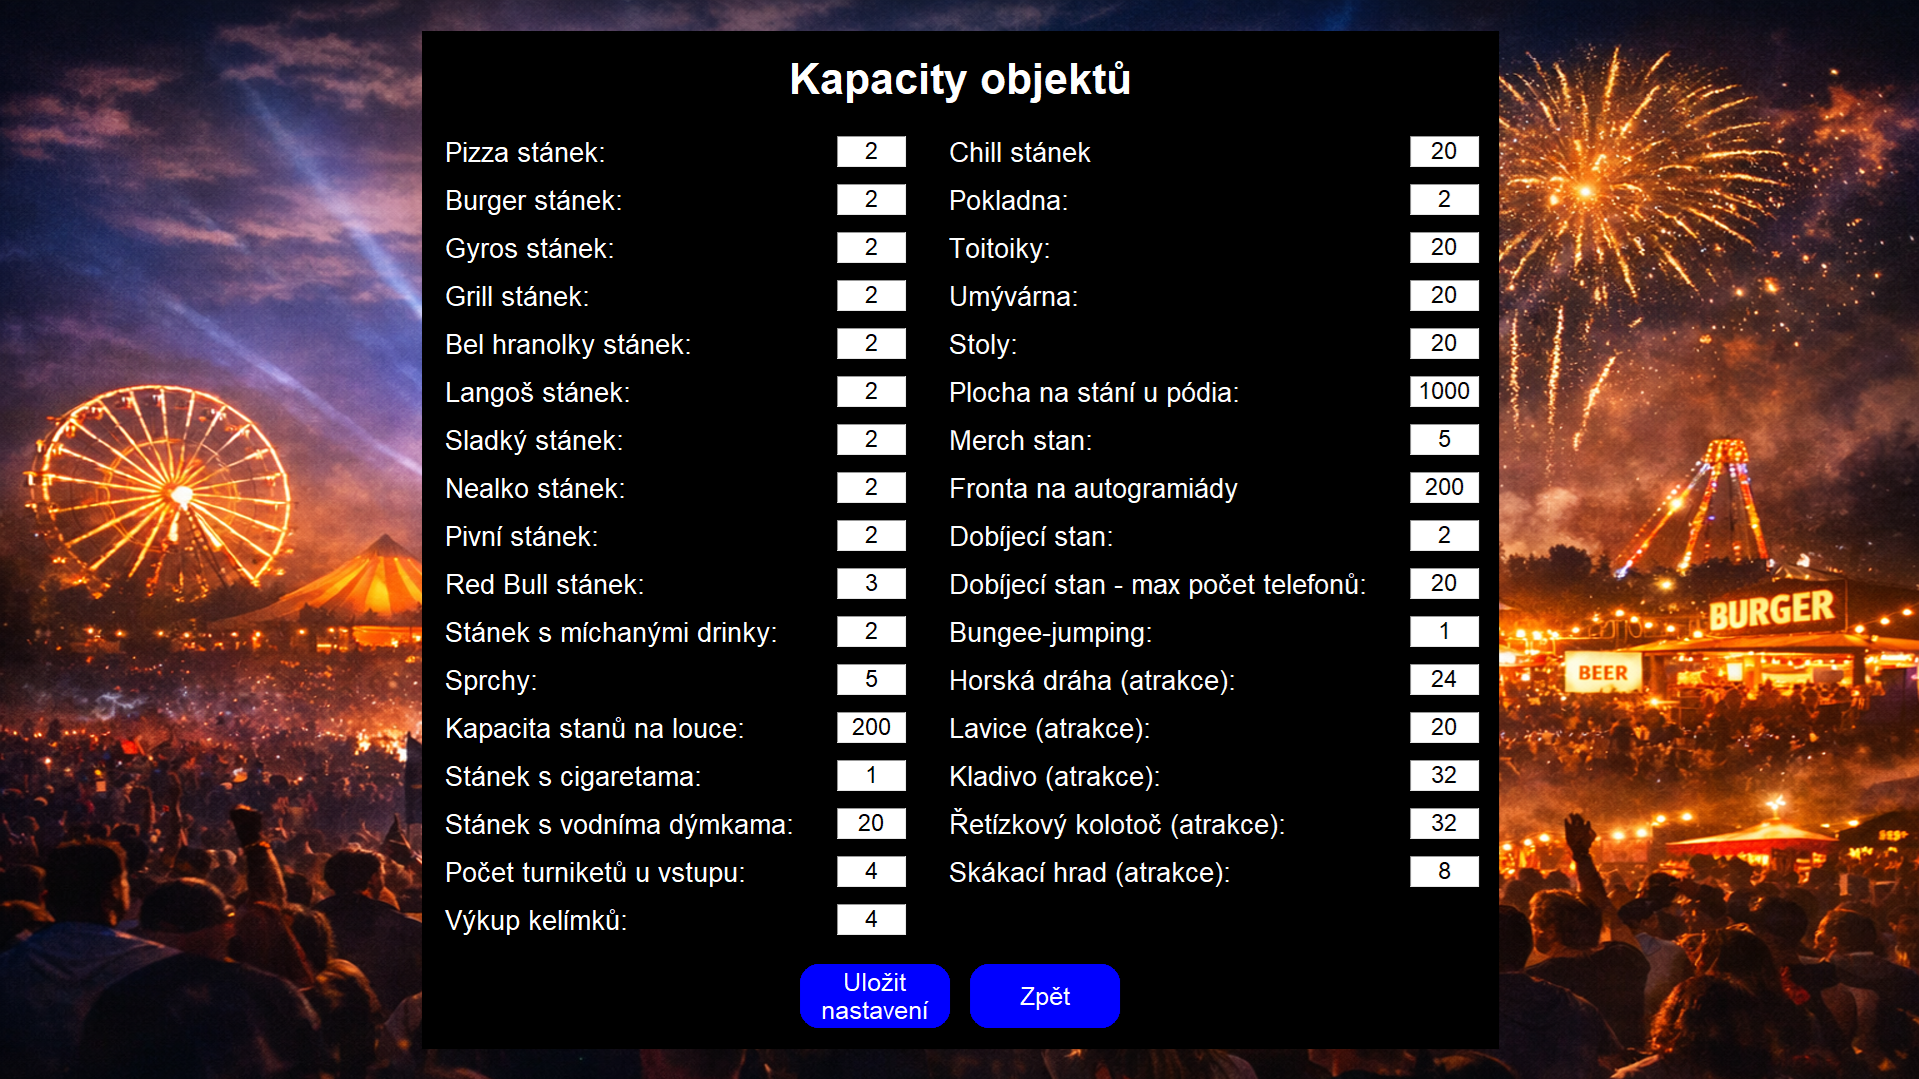
\includegraphics[width=1.0\textwidth]{images/nastaveni_capacity.png}
    \caption{Nastavení kapacit objektů}
    \label{fig:nastaveni_capacity}
\end{figure}

\paragraph{Provozní doba stánků}\hfill\\
Provozní dobu je možné nastavovat u všech stánků, které poskytují služby návštěvníkům, s vyjímkou pokladen. Jednotlivé stánky jsou rozděleny do dvou kategorií, a to na stánky umístěné přímo ve festivalovém areálu a stánky nacházející se mimo areál. Obě skupiny mohou mít odlišnou provozní dobu. Konfigurace provozní doby se provádí v okně zobrazeném na obrázku \ref{fig:nastaveni_otviraci_doby}. Uživatel zde zadává čas otevření a uzavření stánků. Všechny časové hodnoty v nastavení je nutné zadávat ve formátu HH:MM.

\begin{figure}[H]
    \centering
    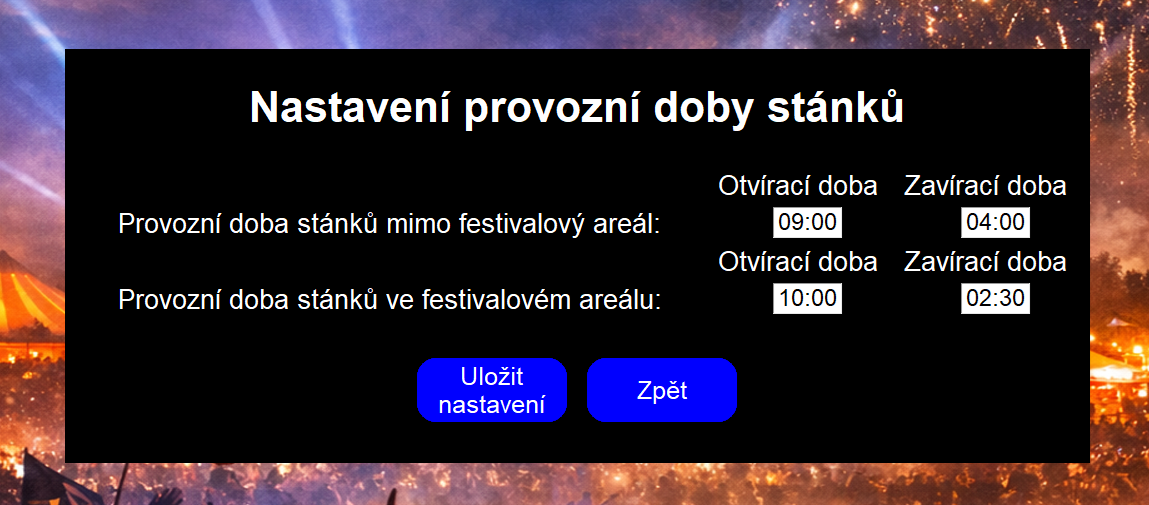
\includegraphics[width=1.0\textwidth]{images/nastaveni_otviraci_doby.png}
    \caption{Nastavení provozní doby stánků}
    \label{fig:nastaveni_otviraci_doby}
\end{figure}

\paragraph{Ceny festivalu}\hfill\\
Cenová konfigurace umožňuje definovat částky, které návštěvníci hradí za jednotlivé služby poskytované v rámci festivalu. Nastavení cen je dostupné prostřednictvím volby \texttt{Ceny festivalu} v základním konfiguračním okně.

\paragraph{Ceny merche}\hfill\\
Během tvorby festivalového areálu může uživatel umístit do plánku také merch stánek, který návštěvníkům umožňuje zakoupit upomínkové předměty jednotlivých kapel i festivalový merch. V této části nastavení lze konfigurovat cenu každého nabízeného předmětu a zároveň určit počet kusů, které budou během simulace k dispozici. Ve výsledcích simulace budou následně uloženy statistiky prodeje, tedy kolik kusů jednotlivých položek bylo prodáno.

Pro zjednodušení modelu mají všechny kapely jednotnou cenu merche, avšak počet prodávaných předmětů se liší podle popularity kapely. Popularnější kapely si sebou vezou více předmětů než méné populární kapely.

\paragraph{Označení objektů}\hfill\\
V rámci nastavení dostupného v okně zobrazeném na obrázku \ref{fig:nastaveni_zvyrazneni} může uživatel konfigurovat barevné označení objektů na festivalovém rovzvržení areálu, jehož vytvoření bude popsáno v následujících podkapitolách. Barevné označení je možné u stánků, plochy určené pro stání před pódiem a louky na stanování ve stanovém městečku. Jednotlivé objekty jsou na festivalovém plánku reprezentovány příslušnými emoji ikonami, některé se však nacházejí uprostřed obdélníku. Obdélníkový tvar se používá u objektů, které obsahují další objekty uvnitř, například louka na stanování, kde se v obedélníku nacházejí jednotlívé stany návštěvníků. V takovém případě se zvýraznění provádí vyplněním plochy uvnitř obdélníku zvolenou barvou. Většina ostatních stánků je zobrazena pouze ikonou, u nichž se zvýraznění realizuje vykreslením barevného kruhu pod ikonou.
Po najetí kurzoru myši na ikonu objektu se nad objektem zobrazí jeho název.

Zvýraznění stánků je rozděleno do čtyř kategorií: \texttt{Stánek je využíván}, \texttt{Malá fronta}, \texttt{Střední fronta} a \texttt{Velká fronta}. První z uvedených kategorií zvýrazní stánek zvolenou barvou ve chvíli, kdy k němu návštěvník přistoupí. Zbývající tři kategorie odpovídají počtu návštěvníků čekajících ve frontě u daného stánku. Uživatel může určit, od jakého počtu osob se má daná úroveň fronty zobrazit, a zároveň zvolit barvu, kterou bude stánek na plánku zvýrazněn. Například lze nastavit, že fronta o velikosti dvaceti osob bude označena jako velká a stánek se v takovém případě zvýrazní červenou barvou. Výběr barvy se provádí pomocí tlačítka \texttt{Vybrat}, které otevře dialog pro volbu barvy. Nalevo od tlačítka se nachází náhled aktuálně zvolené barvy. Stejný princip zvýrazňování je použit také u plochy před pódiem a u louky na stanování, kde může uživatel sledovat návštěvnost jednotlivých kapel nebo míru obsazenosti stanových míst. V těchto dvou případech se hodnoty nezadávají jako počet osob, ale jako procentuální zaplněnost dané plochy.


\begin{figure}[H]
    \centering
    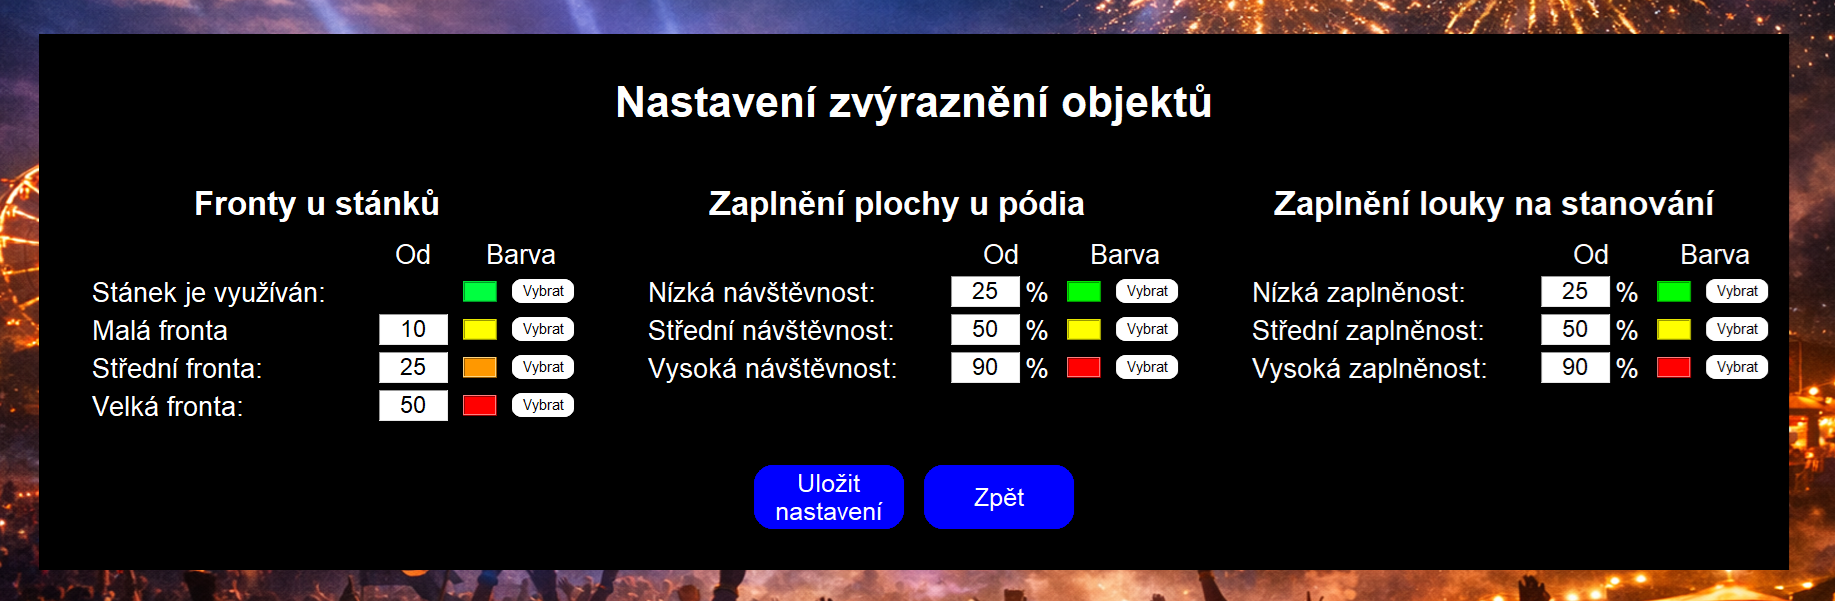
\includegraphics[width=1.0\textwidth]{images/nastaveni_zvyrazneni.png}
    \caption{Nastavení zvýraznění stánků}
    \label{fig:nastaveni_zvyrazneni}
\end{figure}

\subsubsection{Nastavení kapel}
Po nastavení všech parametrů simulace lze pomocí tlačítka \texttt{Pokračovat} přejít k dalšímu kroku, kterým je konfigurace harmonogramu vystoupení kapel. Harmonogram je možné vytvořit ručně, načíst z dříve uloženého souboru, nebo vygenerovat pomocí vestavěného generátoru. Tlačítko \texttt{Pokračovat} ve spodním panelu obrazovky je nyní deaktivované a zpřístupní se až v okamžiku vytvoření, vygenerování či načtení časového harmonogramu kapel.

\paragraph{Generování harmonogramu}\hfill\\
Po kliknutí na tlačítko \texttt{Vygenerování lineupu} se uživatel dostane do nabídky konfigurace generátoru časového harmonogramu (obrázek \ref{fig:nastaveni_generovani_harmonogramu} ). V této části lze nastavit délku vystoupení běžné kapely a \emph{headlinera}, přičemž headlinerem je vždy poslední kapela daného dne. Délka vystoupení headlinera se může v konečném výsledku mírně lišit od hodnoty zadané uživatelem, protože přestávky mezi jednotlivými koncerty jsou zaokrouhlovány dolů na nejbližší násobek deseti minut a vzniklý zbytkový čas je následně přičten k délce vystoupení headlinera. Tato úprava zajišťuje přehlednější časový harmonogram, ve kterém koncerty začínají i končí v přirozenější časy.

Uživatel dále může nastavit délku trvání autogramiád, počet kapel generovaných na každý den, čas začátku prvního koncertu a čas ukončení posledního koncertu daného dne.  Díky dříve zmíněné úpravě času headlinera je dodržen čas začátku prvního a konce posledního koncertu. Program umožňuje, aby koncertní blok přesáhl do následujícího kalendářního dne, přičemž se stále považuje za součást původního festivalového dne. Čas konce posledního koncertu je však omezen nejpozději na 2:00 ráno. Všechna vstupní pole obsahují kontrolu správnosti zadaných hodnot. Při uložení nastavení tlačítkem \texttt{Uložit nastavení}, bez něhož se hodnoty do generování nepromítnou, se ověřuje, zda je konfigurace přípustná. Například mezi jednotlivými koncerty musí být zachována minimálně patnácti minutová přestávka na přestavbu pódia. 

Po nastavení všech hodnot uživatel může vygenerovat časový harmonogram pomocí tlačítka \texttt{Vygenerovat}. Vygenerování následně umožní uložit harmonogram do zvoleného adresáře tlačítkem \texttt{Uložit lineup}.

\begin{figure}[H]
    \centering
    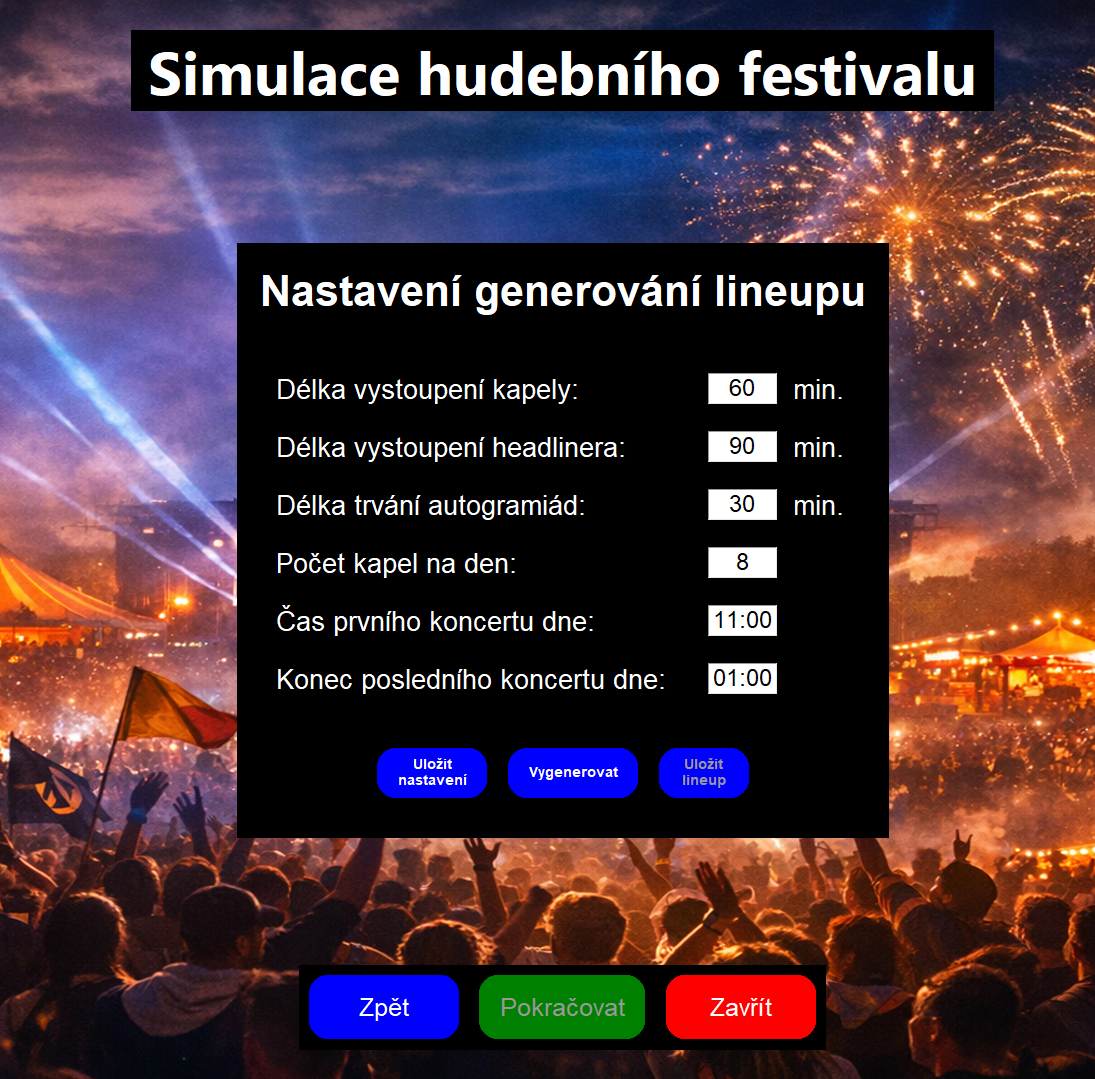
\includegraphics[width=1.0\textwidth]{images/nastaveni_generovani_harmonogramu.png}
    \caption{Nastavení generování časového harmonogramu kapel}
    \label{fig:nastaveni_generovani_harmonogramu}
\end{figure}

Generátor lineupu využívá seznam kapel uložený v souboru \texttt{/data/bands.json}. Každá kapela v tomto souboru obsahuje kromě názvu také atribut \texttt{popularity}, který slouží k určení pořadí kapel v rámci jednotlivých festivalových dnů. Při generování se pro každý den náhodně vybere uživatelem zadaný počet kapel, které jsou následně seřazeny podle popularity. Tímto způsobem je určena i role headlinera, jelikož headlinerem se stává kapela s nejvyšší popularitou. Datový soubor je možné libovolně rozšiřovat o další kapely, případně upravit hodnoty popularity. 

\paragraph{Vytvoření harmonogramu}\hfill\\
Vytvoření časového harmonogramu ručně je možné v části \texttt{Vytvořit lineup}. Tato obrazovka aplikace umožňuje uživateli sestavit časový harmonogram vystoupení kapel manuálně. Rozhraní je rozděleno do jednotlivých festivalových dnů, mezi nimiž lze přepínat pomocí záložek. Každý den obsahuje tabulku, do níž uživatel zadává název kapely, čas začátku a konce koncertu a čas začátku a konce autogramiády. Tímto způsobem lze vytvořit vlastní lineup bez využití generátoru harmonogramu nebo načítání z externího souboru.

Uživatel může vyplnit libovolný počet řádků, minimálně však jeden a maximálně dvanáct řádků, což odpovídá maximálnímu počtu kapel na den i při generování harmonogramu. Je nutné vyplnit všechny hodnoty na daném řádku, a to i v případě, že uživatel neplánuje na festivalu pořádat autogramiády. Jednotlivé časy se navíc nesmí překrývat. Na obrázku~\ref{fig:nastaveni_vytvareni_harmonogramu.png} je znázorněno vyplnění formuláře pro první den festivalu, v němž vystoupí pouze tři kapely. Na rozdíl od automatického generování harmonogramu je při ručním vytvoření možné, aby měl každý festivalový den odlišný počet kapel. Při ručním vytváření harmonogramu se neuvádí popularita kapely, protože pořadí kapel i časy jejich vystoupení určuje uživatel. Popularita je však do interního souboru \texttt{data/lineup} doplněna při ukládání. První kapela získá hodnotu popularity 10 a každá následující kapela v pořadí má popularitu zvýšenou o 10. Tento mechanismus slouží k tomu, aby kapely s vyšší popularitou měly v simulaci větší množství dostupného merche ve stánku s merchandisingem. 

Jakmile je harmonogram nastavený je zpřístupněno tlačítko \texttt{Pokračovat} v dolním panelu obrazovky. Můžeme tedy přejít na editaci festivalového areálu.

\begin{figure}[H]
    \centering
    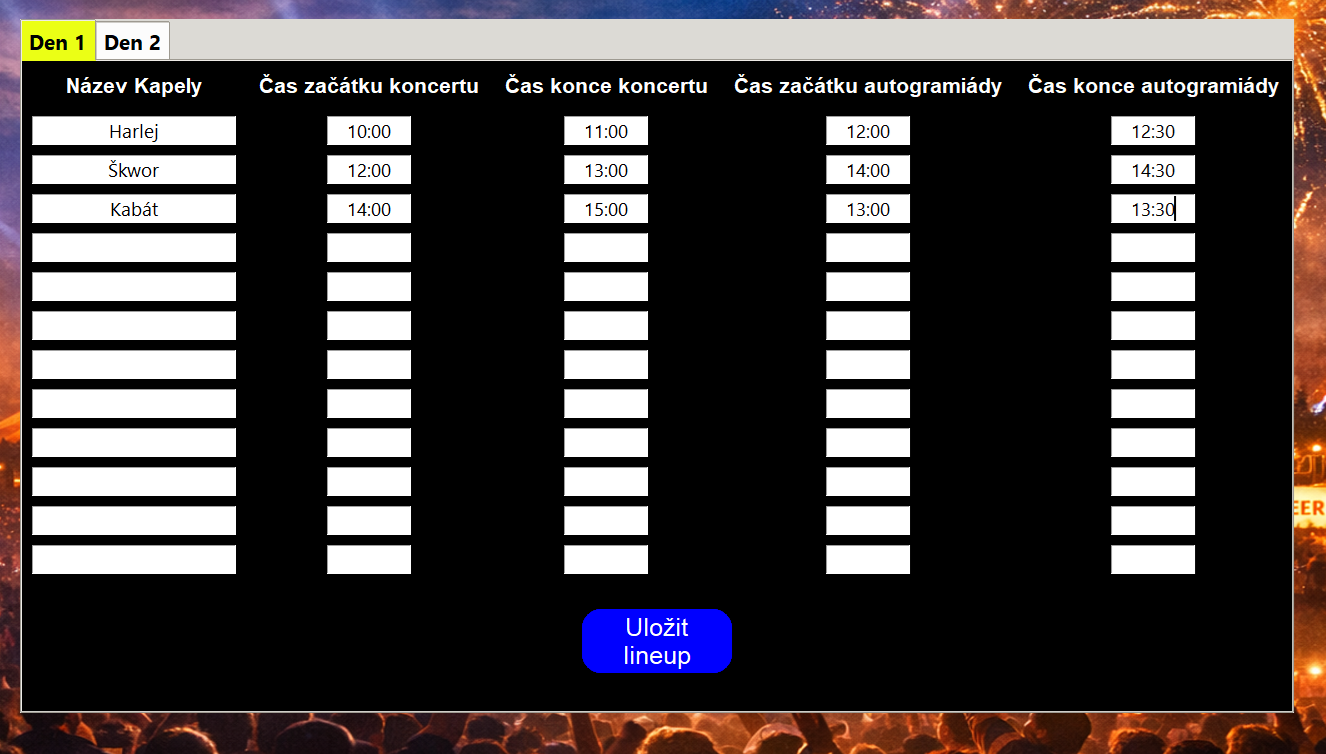
\includegraphics[width=1.0\textwidth]{images/nastaveni_vytvareni_harmonogramu.png}
    \caption{Vytváření časového harmonogramu kapel}
    \label{fig:nastaveni_vytvareni_harmonogramu}
\end{figure}

\subsubsection{Festivalový editor}
Festivalový areál je interně uložen v souboru \texttt{data/festival\_settings}. Pokud se v tomto souboru nachází již dříve vytvořený a validní festivalový areál, je automaticky načten při vstupu do editoru festivalového areálu. V případě, že soubor neobsahuje žádná data nebo neexistuje, je uživateli zobrazen výchozí prázdný canvas.

Editor se skládá ze dvou levých panelů (viz obrázek \ref{fig:editor_leve_panely}), centrálního canvasu a spodní lišty s ovládacími tlačítky. Tlačítko \texttt{Zpět} uživatele přesměruje na předchozí krok, tedy na nastavení kapel. Pomocí tlačítka \texttt{Uložit} lze aktuální podobu areálu uložit. Tlačítko \texttt{Načíst} umožňuje načíst již existující areál ze souboru. Funkce \texttt{Smazat} vymaže celý canvas a umožní uživateli začít s tvorbou areálu od začátku. Tlačítko \texttt{Start} přepne aplikaci do simulačního režimu a zároveň automaticky uloží festivalový areál do již zmíněného interního souboru.

Pro úspěšné přepnutí do simulačního režimu je nutné splnit minimální požadavky na strukturu festivalového areálu. Musí existovat zóna \texttt{Spawn\_zóna}, do níž návštěvníci při zahájení simulace přicházejí. Dále musí být na festivalu umístěn alespoň jeden stánek s jídlem a nealkoholickým pitím, (jakýkoliv stánek s pitím kromě stánku \texttt{Míchané drinky}). Součástí areálu musí být také bankomat, pokladna, toalety (objekt typu \texttt{toitoi}) a v zóně \texttt{Festivalový areál} musí být umístěno pódium. Všechny ostatní objekty jsou volitelné. Poslední podmínkou pro úspěšný přechod do simulačního režimu je, že jednotlivé zóny musí být navzájem propojeny. Následující část textu vysvětluje, jak tyto požadavky splnit. Napřed si ale představme jednotlivé zóny a jejich účel.

\paragraph{Festivalové zóny}\hfill\\
Zóny představují logické rozdělení festivalového areálu, přičemž každá z nich má specifický účel. Aplikace poskytuje celkem šest typů zón. \texttt{Spawn zóna} je místem, na které návštěvníci při zahájení simulace přicházejí. Jedná se o jejich výchozí bod. Tato zóna nemá žádný další účel a není do ní možné umisťovat objekty. \texttt{Vstupní zóna} se nachází před hlavním oploceným areálem a představuje prostor, do něhož se mohou návštěvníci dostat i bez vstupenky. Slouží jako přirozený předstupeň hlavního areálu a umožňuje oddělit volně přístupné části festivalu od těch, které vyžadují kontrolu vstupních pásků. \texttt{Stanové městečko} je určeno pro kempování návštěvníků a poskytuje prostor pro stanování a sprchy, což je využitelné zejména při vícedenních festivalech. \texttt{Zábavní zóna} obsahuje různé atrakce a rozšiřuje nabídku aktivit mimo hlavní hudební program. \texttt{Chill zóna} slouží k odpočinku návštěvníků. Může, ale nemusí být umístěna uvnitř festivalového areálu.  \texttt{Festivalový areál} je hlavní zóna, v níž se nachází pódium, merch stánek, prostor pro autogramiády a další prvky, které vyžadují kontrolu vstupních pásků. Jedná se o centrální část festivalu, kde probíhá hlavní program a kde se návštěvníci zdržují nejčastěji.

\begin{figure}[H]
    \centering
    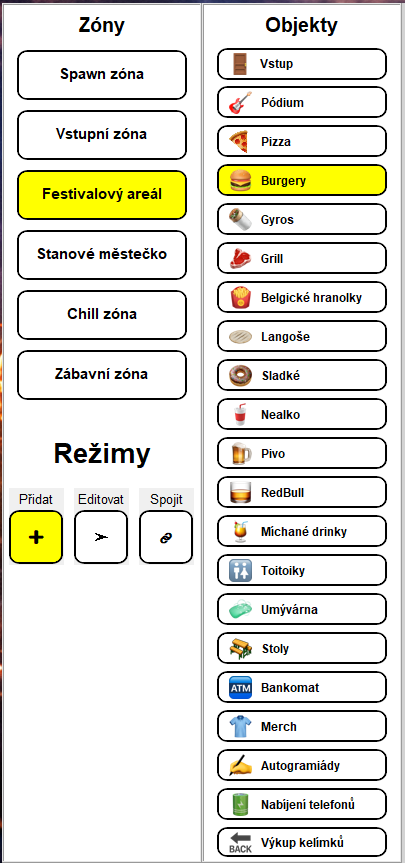
\includegraphics[width=0.4\textwidth]{images/editor_leve_panely.png}
    \caption{Panely pro vytváření festivalového areálu}
    \label{fig:editor_leve_panely}
\end{figure}

\paragraph{Vytváření rozložení festivalového areálu}\hfill\\
Levý sloupec ovládacího panelu obsahuje výběr zón a režimů editace. Pravý sloupec zobrazuje seznam objektů, které je možné do jednotlivých zón umístit. Aktuálně vybraná zóna, režim a objekt jsou zvýrazněny žlutou barvou. Editor nabízí tři režimy práce: \texttt{Přidat}, \texttt{Editovat} a \texttt{Spojit}.

Režim \texttt{Přidat} slouží k vytváření zón a vkládání objektů do zón. Každá zóna může být na festivalu pouze jednou a vytváří se kliknutím a tažením myši, čímž vznikne modrý obdélník představující její ohraničení. Vybraný objekt lze umístit pouze do plochy odpovídající zóny a přidává se prostým kliknutím do jejího prostoru. 

Režim \texttt{Editovat} umožňuje upravovat hranice zóny tažením myši za její hranu a rovněž přesouvat vložené objekty kliknutím, držením a tažením myši. Zóny a objekty vybrané v editačním režimu jsou zvýrazněny červeným ohraničením. V tomto režimu lze také kliknout na spojnici mezi zónami, která se následně rovněž zvýrazní červeně.

V posledním kroku je nutné vytvořené zóny propojit v režimu \texttt{Spojit}. Není nutné spojit každou zónu s každou, ale musí být zajištěno, aby byla každá zóna dosažitelná, tedy aby vznikl neorientovaný graf. Režim spojení funguje tak, že uživatel nejprve klikne na jednu zónu a poté na druhou. Po druhém kliknutí se mezi nimi vytvoří spojovací čára vedoucí od středu nejbližších hran obou zón.

Zóna \texttt{Festivalový areál} může být propojena dvěma způsoby. Prvním je standardní propojení popsané výše, které umožňuje volný pohyb návštěvníků mezi danou zónou a festivalovým areálem. Tento způsob vyjadřuje že se propojená zóna nachází uvnitř festivalového areálu. Typickým příklad použití může být například propojení mezi zónami \texttt{Festivalový areál} a \texttt{Chill zóna}. Druhým způsobem je propojení přes objekt vstupu. V takovém případě musí návštěvníci při přechodu projít přes vstupní kontrolu, kde se ověřuje, zda mají vstupní pásek. Pro tento typ propojení je nutné v režimu \texttt{Přidat} vložit do festivalového areálu objekt \texttt{Vstup}, který lze umístit pouze na hranu zóny \texttt{Festivalový areál}. Následně lze v režimu \texttt{Spojit} kliknout na vstup a poté na zónu, kterou má vstup propojit.

Objekt vstupu lze v editačním režimu přesouvat po hraně zóny pouze tehdy, pokud není spojen s žádnou jinou zónou. Hranou zóny lze pohybovat pouze v případě, že na ní není umístěn žádný vstup a zároveň se v její těsné blízkosti nenachází žádný objekt.

Vybraný objekt, zónu nebo spojení mezi zónami lze smazat stiskem klávesy \texttt{Delete}. Smazáním vstupu se odstraní všechna jeho propojení. Smazáním zóny se odstraní všechny objekty uvnitř zóny i všechna její spojení. Na obrázku \ref{fig:editor_festivalovy_areal} je ukázka možného výsledného rozložení festivalového areálu. Po vytvoření areálu můžeme pokračovat do simulační části aplikace stiskem tlačítka \texttt{Start}.

\begin{figure}[H]
    \centering
    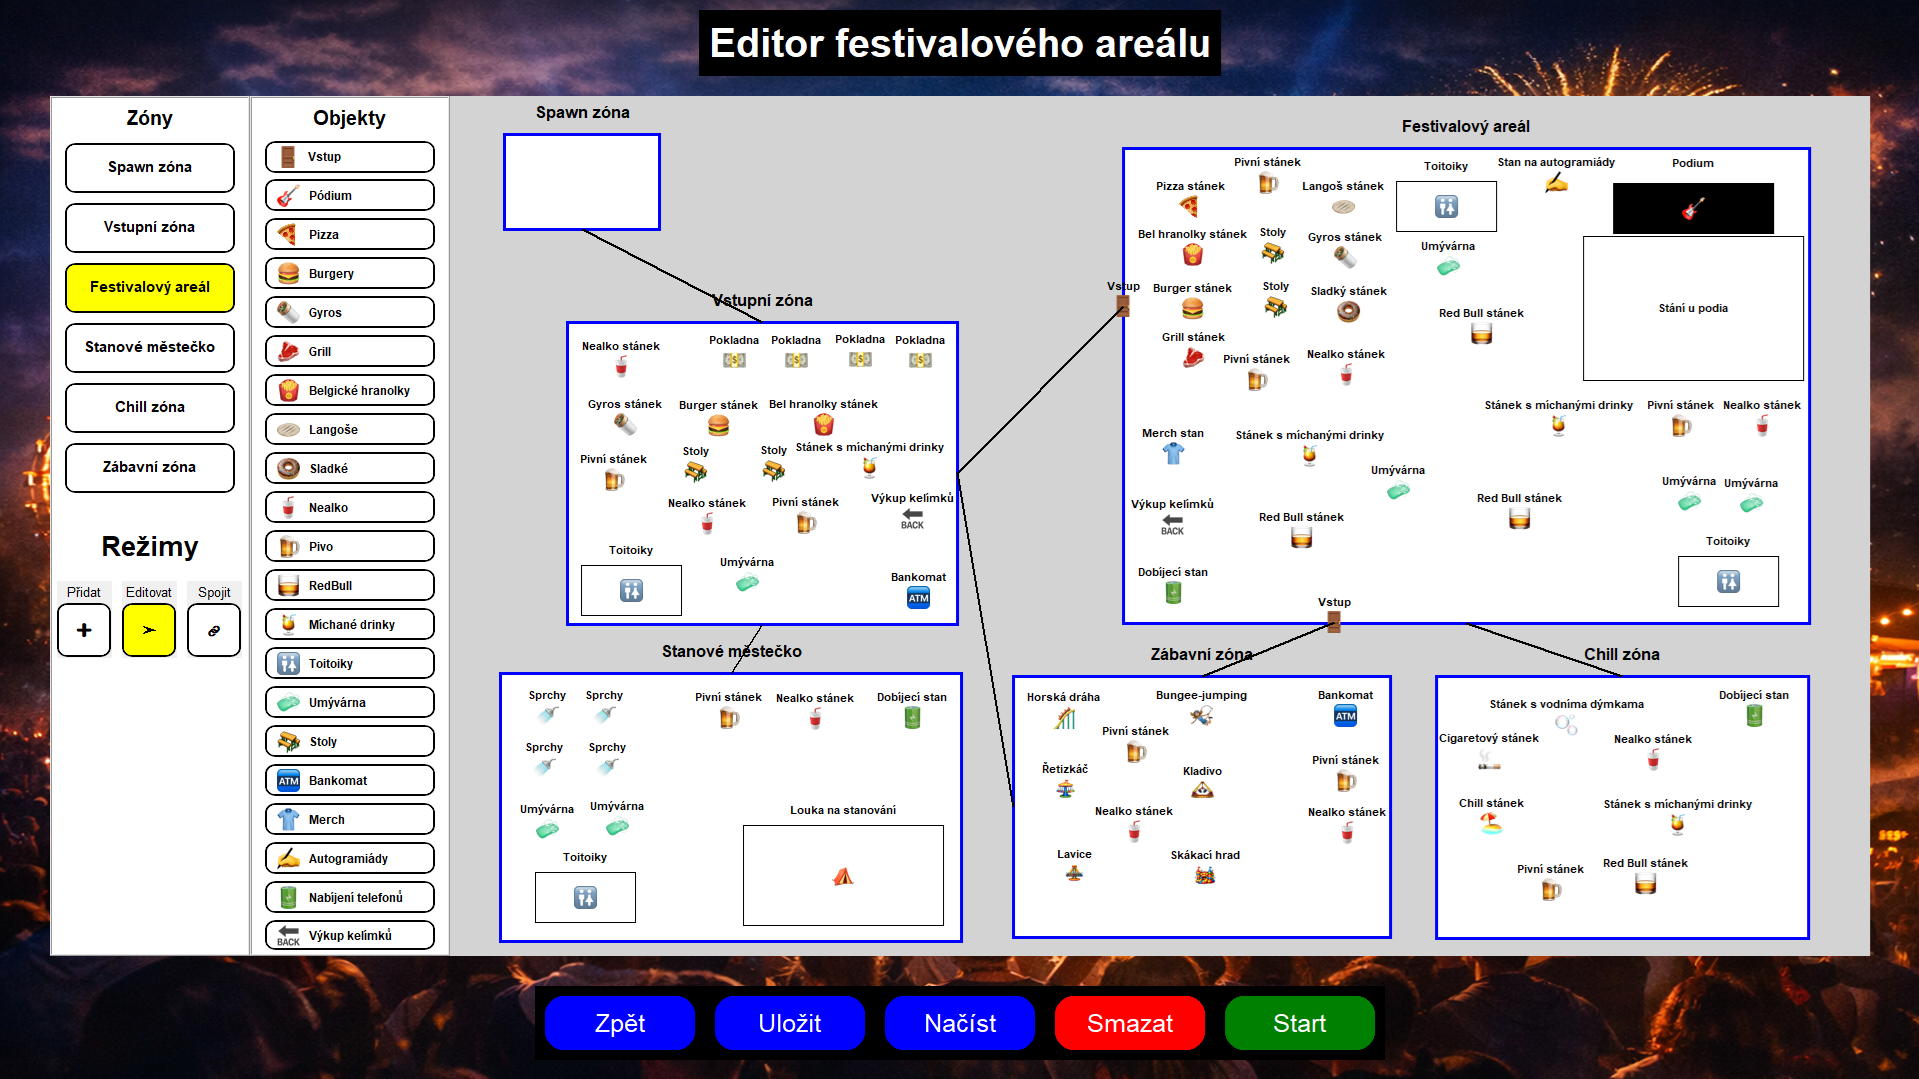
\includegraphics[width=1.0\textwidth]{images/editor_festivalovy_areal.png}
    \caption{Ukázka možného rozložení festivalového areálu}
    \label{fig:editor_festivalovy_areal}
\end{figure}

\subsubsection{Simulační režim}
Při přechodu do simulačního režimu probíhá generování návštěvníků, z tohoto důvodu může při větším počtu návštěvníků přepnutí trvat několik vteřin. V simulačním režimu se u každé zóny v levém horním rohu zobrazí ukazatel aktuálního počtu návštěvníků v dané zóně. Změní se také levý panel. V jeho záhlaví najdeme informaci o aktuálním simulačním času a aktuálním festivalovém dnu. Pod záhlavím se nachází horní část panelu, ta nyní zobrazuje detailní informace o jednotlivých stáncích. Spodní část slouží jako výpis událostí, které se v simulaci právě odehrávají. Detail konkrétního objektu si uživatel zobrazí kliknutím na jeho ikonu. Tyto funkcionality budou podrobněji popsány později v podkapitole \texttt{Plynulá simulace}. V simulačním režimu není možné měnit rozmístění objektů ani jinak upravovat rozložení areálu. Současně se změní i spodní ovládací lišta, jejíž simulační verzi lze vidět na obrázku \ref{fig:simulace_spodni_lista}. Obsahuje mimo jiné tlačítko \texttt{Ukončit}, které simulaci ukončí a vrátí uživatele zpět do editoru.

\begin{figure}[H]
    \centering
    
\includegraphics[width=1.0\textwidth]{images/simulace_spodni_lista.png}
    \caption{Spodní lišta v simulačním režimu}
    \label{fig:simulace_spodni_lista}
\end{figure}

\paragraph{Rychlá simulace}\hfill\\
Spodní lišta nabízí dva základní způsoby spuštění simulace. Prvním z nich je rychlá simulace, aktivovaná tlačítkem \texttt{Rychlá simulace}. V tomto režimu proběhne celá simulace zrychleně na pozadí a uživatel si následně může zobrazit dostupné výsledky dostupné ve složce \texttt{outpusts}.

\paragraph{Plynulá simulace}\hfill\\
Druhým způsobem je plynulá simulace, která se spouští tlačítkem \texttt{Plynulá simulace}. V tomto režimu běží simulace v reálném čase, kde jedna minuta simulace odpovídá jedné vteřině skutečného času. Uživatel může průběžně sledovat měnící se počty návštěvníků v jednotlivých zónách, barevné zvýraznění objektů při vzniku front či jejich vytíženosti, detaily objektů a také živé výpisy událostí ze simulace. Logy jsou zobrazovány s mírným zhruba minutovým zpožděním, protože vznikají během simulace dané minuty, ale jejich vykreslení probíhá až při následující aktualizaci GUI. Na obrázku \ref{fig:plynula_simulace_zacatek} je zachycen začátek plynulé simulace při nastavení festivalu na dva dny, začátek simulace v 8:00 a s celkovým počtem jednoho tisíce návštěvníků. V levém panelu je v horní části zobrazen detail \texttt{Pizza stánku}, u něhož se aktuálně nachází jeden návštěvník ve frontě a dva návštěvníci jsou právě obsluhováni. Zajímavým prvkem je červené zvýraznění louky na stanování ve stanovém městečku, které signalizuje vyčerpání kapacity pro umístění dalších stanů. V zóně \texttt{festivalový areál} lze zároveň pozorovat, že stánky obsluhující návštěvníky mají šedé ikony, což značí, že jsou v aktuálním času simulace zavřené. Po otevření detailu stánku \texttt{Pivní stánek} nacházejícího se v zóně \texttt{Festivalový areál} můžeme vidět, že otevření tohoto stánku nastane za osmnáct minut simulovaného času (viz obrázek \ref{fig:plynula_simulace_zavreny_stanek}).

\begin{figure}[H]
    \centering
    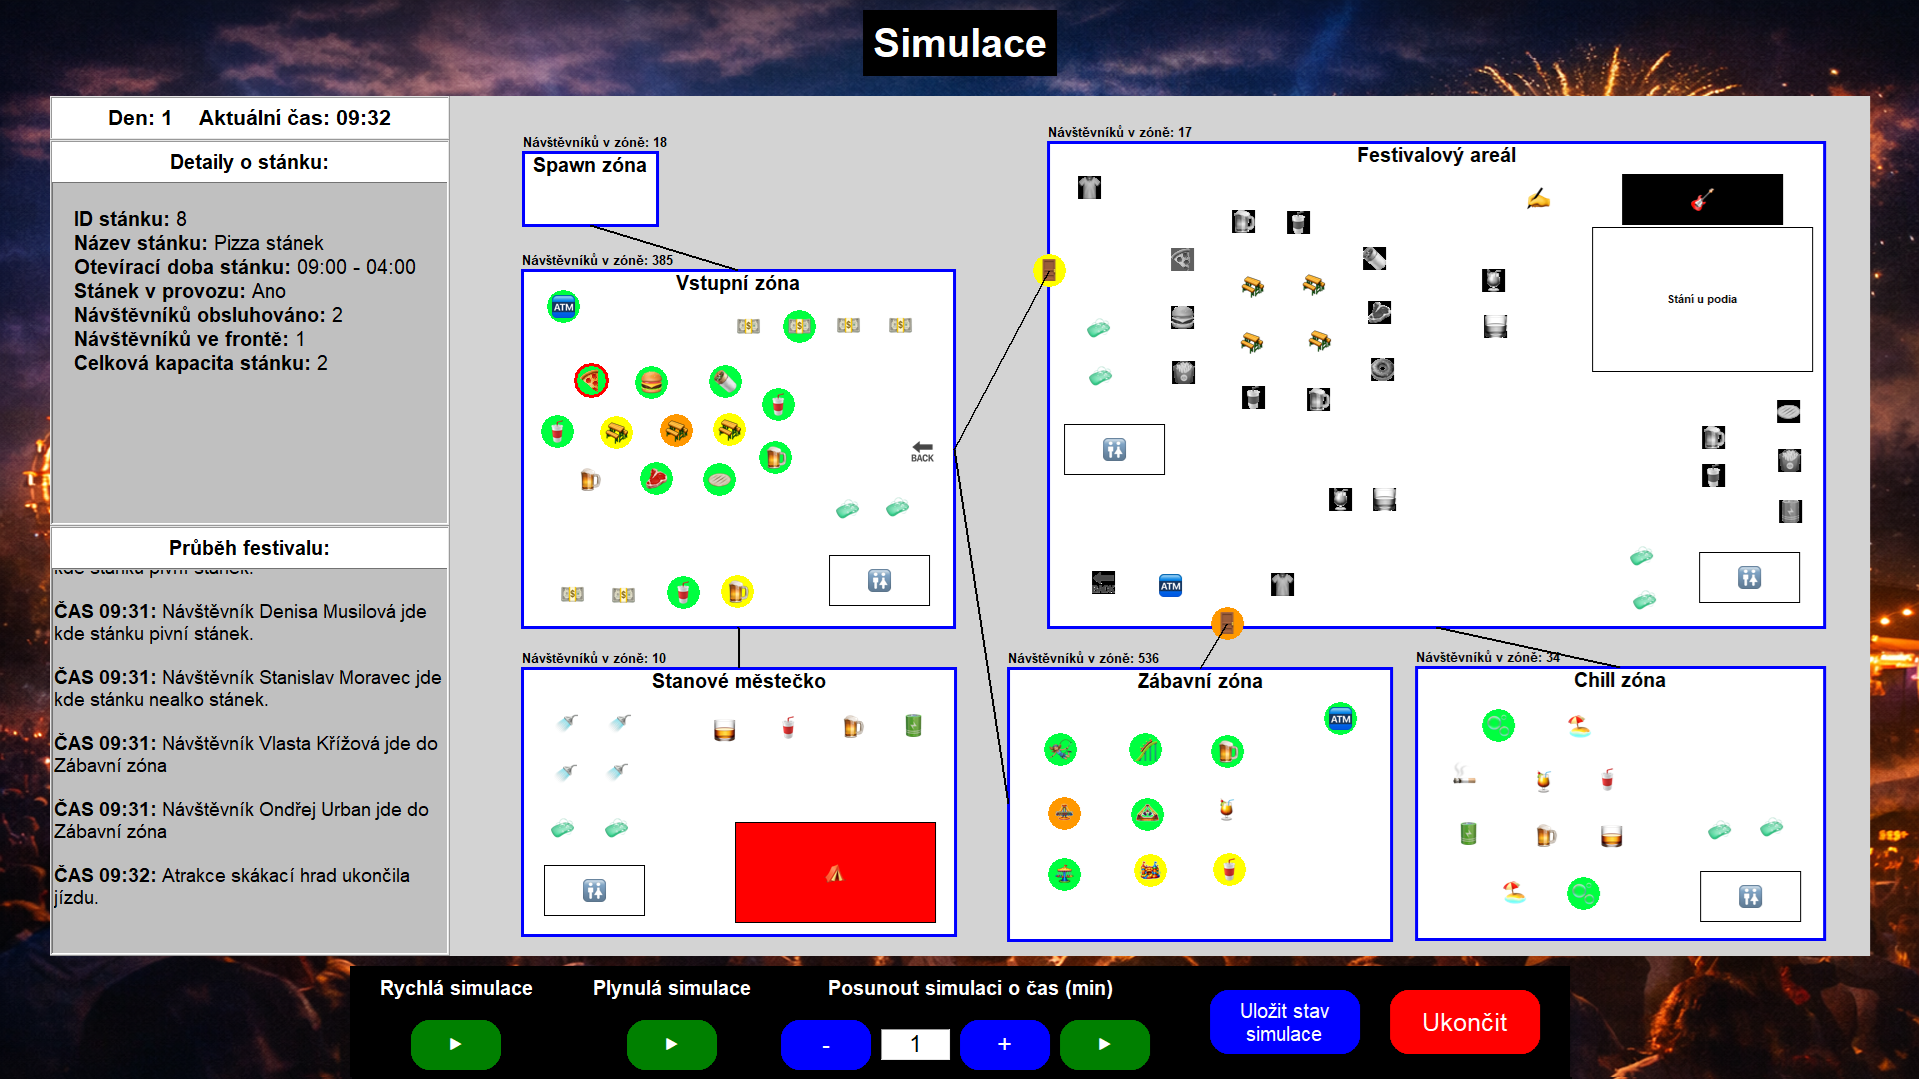
\includegraphics[width=1.0\textwidth]{images/plynula_simulace_zacatek.png}
    \caption{Ukázka plynulé simulace}
    \label{fig:plynula_simulace_zacatek}
\end{figure}

\begin{figure}[H]
    \centering
    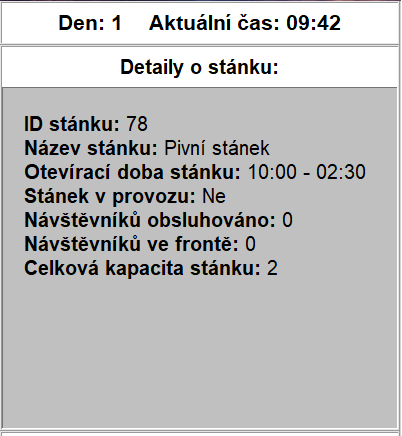
\includegraphics[width=0.5\textwidth]{images/plynula_simulace_zavreny_stanek.png}
    \caption{Ukázka plynulé simulace}
    \label{fig:plynula_simulace_zavreny_stanek}
\end{figure}

Lišta dále nabízí možnost posunout simulaci o zadaný čas prostřednictvím rozhraní \texttt{Posunout simulaci o čas}. To obsahuje vstupní pole přijímající pouze celočíselné hodnoty. Po stisknutí zeleného tlačítka se simulace posune o zadaný počet minut dopředu. Hodnotu je možné upravovat také pomocí tlačítek po stranách vstupního pole, která umožňují její zvýšení či snížení o jednu jednotku.

Během běhu plynulé simulace není možné přejít na rychlou simulaci a posovouvat simulační čas prostřednictvím rozhraní \texttt{Posunout simulaci o čas}, s výjimkou tlačítka \texttt{Plynulá simulace}, kterým lze simulaci pozastavit. Uživatel může simulaci kdykoliv spustit, zastavit, prozkoumat aktuální stav a opět pokračovat. Zbytek simulace lze případně dokončit zrychleně pomocí rychlé simulace, pokud je simulace pozastavená.

Během plynulé simulace lze kdykoliv uložit aktuální stav simulace do souboru \texttt{outputs/simulation\_states.json} pomocí tlačítka \texttt{Uložit stav simulace}.

\subsection{Výsledky simulace}
Po dokončení simulace se zobrazí informativní zpráva oznamující její úspěšné dokončení. Po stisknutí tlačítka \texttt{Zavřít} je uživatel přesměrován zpět na úvodní obrazovku, odkud může zahájit novou simulaci.

\section{Možná rozšíření}
Aplikace v současné verzi využívá několik zjednodušení, která byla zvolena s ohledem na rozsah práce a přehlednost výsledného modelu. Je však zřejmé, že by bylo možné doplnit mnoho dalších funkcí a objektů, které by model dále rozšířili. Uvedený seznam možných rozšíření proto není konečný a představuje pouze nejvýznamnější směry, které se během vývoje nabízely.

\begin{itemize}

\item \textbf{Více typů zón} – Aktuální verze aplikace umožňuje použít každý typ zóny pouze jednou. Do budoucna by bylo možné rozšířit editor o více instancí stejných zón, například několik samostatných chill zón, více vstupních zón nebo více stanových městeček. Zároveň by bylo možné přidat i nové typy zón, jako například VIP zónu, technické zázemí, backstage, parkoviště, nebo zónu pro zdravotní službu. Tím by bylo možné modelovat rozsáhlejší a realističtější festivalové areály.

\item \textbf{Více typů objektů} – Současná implementace obsahuje základní sadu objektů nezbytných pro běh simulace a typických pro téměř jakýkoliv hudební festival. Model by bylo možné rozšířit o další objekty, které by nabízeli návštěvníkům více dostupných aktivit. Zároveň je v aktuální verzi možné umístit pouze jedno pódium. Rozšíření o více pódií by umožnilo simulovat paralelní koncertní program.

\item \textbf{Prvky infrastruktury} – V aktuální verzi simulace nejsou zahrnuty prvky interní infrastruktury festivalu, které mají zásadní vliv na jeho provoz. Do budoucna by bylo možné doplnit například zaměstnance festivalu, jako jsou členové bezpečnostní služby, zdravotníci, technici, dobrovolníci či pracovníci úklidu. Další možností je přidání objektů typu backstage, technické zázemí, skladovací prostory nebo servisní stanoviště. Tyto prvky by umožnily simulovat logistiku festivalu, pohyb personálu a jejich interakci s návštěvníky.

\item \textbf{Ekonomický model simulace} – Současná verze aplikace pracuje pouze se základními cenami služeb a merchandisingu. Rozšíření o komplexnější ekonomický model by umožnilo sledovat finanční stránku festivalu, například celkové náklady na kapely, provoz stánků, pronájem areálu či mzdy zaměstnanců. Zároveň by bylo možné vyhodnocovat zisk jednotlivých stánků, celkový výnos festivalu, vliv nastavení cen na chování návštěvníků. Takové rozšíření by poskytlo detailnější pohled na ekonomickou udržitelnost festivalu.

\item \textbf{Vnější vlivy} – Simulaci by bylo možné rozšířit o faktory, které ovlivňují průběh festivalu z vnějšího prostředí. Patří sem například počasí, které může ovlivnit návštěvnost, délku front nebo využití jednotlivých zón. Dalším příkladem jsou mimořádné události, bezpečnostní incidenty či technické poruchy. Tyto vlivy by umožnily simulovat krizové scénáře a testovat odolnost festivalového provozu.

\item \textbf{Optimalizace vizuálního běhu simulace} – Plynulá simulace v aktuální implementaci průběžně aktualizuje vizuální stav celého festivalu, mění barvy a ikony objektů podle jejich vytížení, zobrazuje logy událostí a průběžně aktualizuje počty lidí v jednotlivých zónách. V kombinaci s Tkinterem, který není navržen pro časté a rozsáhlé aktualizace velkého množství grafických prvků, vede tento přístup k výraznému zatížení hlavního vlákna aplikace. Výsledkem je snížená plynulost, opožděné vykreslování a celkové sekání simulace při vyšším počtu návštěvníků. Oproti tomu rychlá simulace probíhá bez grafického rozhraní a díky absenci vizuálního vykreslování běží i při vysokém počtu návštěvníků zcela plynule. Možným rozšířením by mohlo být využití modernějších grafických knihoven, například PyGame nebo Kivy. Tyto úpravy by umožnily zachovat vizuální podobu simulace, ale zároveň výrazně zvýšit její plynulost a škálovatelnost.
\end{itemize}

\section{Závěr}







\newcommand{\BibLaTeX}{\textsc{Bib}\LaTeX}

% \noindent\textcolor{red}{\LARGE Upozornění: Následující text
%   dokumentace stylu, vyjma přílohy~\ref{sec:ObsahData}, je rozpracovaná
%   a (značně) neúplná verze!!!}

\section{Styly pro psaní bakalářských a diplomových prací}
Toto jsou styly pro psaní bakalářských a diplomových prací přes typografický systém \LaTeX{}, tedy \textbf{kistyles}.

\subsection{Požadavky a podprovaná prostředí}
Sada balíku \textbf{kistyles} podporuje následující distribuce systému \LaTeX{}:
\begin{itemize}
\item \TeX{} Live.
\end{itemize}

Jsou podporovány všechny výstupní ovladače, tedy jak \textbf{dvi}, tak \textbf{pdf} i \textbf{ps}. Funkčnost zmiňovaných distribucí byla ověřena na několika operačních systémech, mezi které patří:
\begin{enumerate}
\item Windows $8.1$,
\item Archlinux,
\item Debian GNU/Linux.
\end{enumerate}

Důrazně se doporučuje používat aktuální verzi dané distribuce systému \LaTeX{}.

%%%  Po přeložení programem CSLaTeX (třikrát) je potřeba použít
%%%  program DVIPS a takto získaný PostScriptový soubor vytisknout
%%%  na PostScriptové tiskárně nebo pomocí programu GhostScript.
%%%
%%%  Rovněž je možné použít program DVIPDFM a vytvořit z dokumentu
%%%  soubor ve formátu PDF včetně hypertextových odkazů.

\subsection{Přepínače}
Styl kidiplom je z hlediska uživatele zastoupen ekvivalentně nazvanou třídou, kterou je třeba volat na záčátku dokumentu:
\begin{kicode}{TeX}{}{Volání třídy \textbf{kidiplom}}
\documentclass[
  master,
  program=ainfvs,
  printversion,
  biblatex,
  language=english,
  font=sans,
  figures=false,
  tables=false,
  theorems,
  sourcecodes,
  joinlists,
  glossaries,
  index,
  encoding=utf8,
  bibencoding=utf8
]{kidiplom}
\end{kicode}

Následuje přehled přepínačů, je vždy uvedeno jméno přepínač, včetně výchozí hodnoty. Přepínače uvádí tabulka \ref{tab:prepinace}.

%\begin{table}
\begin{center}
\begin{longtable}{>{\bfseries}l >{\ttfamily}c L{8cm}}
\caption{Seznam přepínačů}\label{tab:prepinace}\\
  {\normalfont Přepínač} & {\normalfont Výchozí hodnota} & {\normalfont Popis} \\
\hline
master & false & Povolí nebo zakáže režim diplomové práce. Výchozí režim je tedy bakalářská práce. \\

printversion & false & Je-li zapnuto, pak budou odkazy vysázeny optimalizovaně pro knižní sazbu. Tuto volbu je nutno použít pro tisk práce. \\

biblatex & false & Zapne sazbu bibliografie přes balík \BibLaTeX{}. \\

language & czech & Jazyk textu práce. Možné hodnoty jsou \textbf{czech},
\textbf{english} a \textbf{slovak}. \\

font & serif & Zapne či vypne podporu pěkného bezpatkového fontu. Možné hodnoty jsou:\newline
\begin{description}\setlength{\itemsep}{-1ex}
\item[serif] Patkové písmo (Computer Modern).
\item[sans] Bezpatkové písmo (Iwona).
\end{description} \\[-3ex]

figures & true & Je-li zapnuto, pak v seznamech položek bude zahrnut seznam obrázků. \\

tables & true & Je-li zapnuto, pak v seznamech položek bude zahrnut seznam tabulek. \\

theorems & false & Je-li zapnuto, pak v seznamech bude zahrnut seznam teorémů. \\

sourcecodes & false & Je-li zapnuto, pak v seznamech bude zahrnut seznam zdrojových kódů. \\

%%% Argument `joinlists' způsobí zřetězení seznamů obrázků, tabulek,
%%% vět a zdrojových kódů. Není-li použít, všechny seznamy jsou
%%% uvedeny na samostatných stránkách.

joinlists & true & Je-li zapnuto, pak seznamy obrázků, tabulek, vět a
zdrojových kódů sázené za obsahem nebudou rozděleny na samostatné stránky. \\

glossaries & false & Je-li zapnuto, pak na konci dokumentu bude vysázen seznam zkratek. \\

index & false & Zapíná podporu sazby rejstříku. \\

%%  'encoding=kódování' pro kódování tohoto a vložených zdrojových
%%  textů v kódování jiném než výchozím utf8
encoding & utf8 & Kódování souboru dokumentu, doporučuje se ponechat výchozí hodnotu. \\

bibencoding & utf8 & Kódování souboru bibliografie. Tato volba má
smysl pouze, pokud je použita bibliografie skrze balíček \BibLaTeX{}. \\

program & \vtop{\hbox{\strut infpvs}\hbox{\strut ainfvs}} & Specifikuje studijní program/obor (specializaci):\newline
\begin{description}
\item[infoi] Informatika (Obecná informatika)\,--\,bakalářský i navazující magisterský,
\item[infpvs] Informatika (Programování a vývoj software)\,--\,bakalářský,
\item[itp] Informační technologie\,--\,bakalářský, prezenční forma,
\item[itk] Informační technologie\,--\,bakalářský, kombinovaná forma,
\item[infui] Informatika (Umělá inteligence)\,--\,navazující magisterský,
\item[ainfvs] Aplikovaná informatika (Vývoj software)\,--\,navazující magisterský,
\item[ainfpst] Aplikovaná informatika (Počítačové systémy a technologie)\,--\,navazující magisterský,
\item[infv] Informatika pro vzdělávání\,--\,bakalářský,
\item[uinf] Učitelství informatiky pro střední školy\,--\,navazující magisterský,
\item[binf] Bioinformatika\,--\,bakalářský i navazující magisterský,
\item[inf] Informatika (bez specializací)\,--\,bakalářský i navazující magisterský,
\item[ainfp] Aplikovaná informatika (bez specializací)\,--\,bakalářský, prezenční forma,
\item[ainfk] Aplikovaná informatika (bez specializací)\,--\,bakalářský, kombinovaná forma,
\item[ainf] Aplikovaná informatika (bez specializací)\,--\,navazující magisterský.
\end{description}
\end{longtable}
\end{center}
%\end{table}

\subsection{Geometrie stránky}
Tento styl používá list velikosti $A4$. Pro sazbu prací je třeba použít jednostrannou sazbu. Levý okraj je rozšířen s ohledem na vazbu výsledné knižní podoby práce.

\section{Sazba částí dokumentu}
\subsection{Sazba úvodní strany či obsahu}
Vysázení všech podstatných částí úvodu práce obstará makro \kiinlinecode{TeX}{!}{\\maketitle}. Pro správné vysázení všech částí a meta-informací je potřeba použí makra \kiinlinecode{TeX}{!}{\\title}, \mbox{\kiinlinecode{TeX}{!}{\\author}} a další. Jejich přehled lze najít ve zdrojovém souboru tohoto dokumentu. V případě použítí \textbf{pdf} výstupu se generuje i dodatečná hlavička souboru s meta-informacemi jako je autor dokumentu, název práce či dalšími.

\subsection{Závěry}
Závěr práce by se měl poskytnout jak v původním jazyce práce, tak v jazyce anglickém. Pro sazbu závěru jsou k dispozici příslušná makra. Berte na vědomí, že v anglickém závěru se aktivuje plně anglická sazba se všemi konvencemi. Tedy je třeba používat anglické uvozovky a další správné typografické prvky.

\begin{kicode}{TeX}{}{Sazba závěrů}
% Tiskne český závěr práce.
\begin{kiconclusions}
Závěr práce v \uv{českém} jazyce.
\end{kiconclusions}

% Tiskne anglický závěr práce.
\begin{kiconclusions}[english]
Thesis conclusions written in \uv{English}.
\end{kiconclusions}
\end{kicode}

\subsection{Matematika}
Pro sazbu matematiky je k dispozici sada standardních maker.
$$\langle f \rangle, \lfloor g \rfloor,
\lceil h \rceil, \ulcorner i \urcorner$$

$$\left\{\frac{x^2}{y^3}\right\}$$

$$
A_{m,n} =
 \begin{pmatrix}
  a_{1,1} & a_{1,2} & \cdots & a_{1,n} \\
  a_{2,1} & a_{2,2} & \cdots & a_{2,n} \\
  \vdots  & \vdots  & \ddots & \vdots  \\
  a_{m,1} & a_{m,2} & \cdots & a_{m,n}
 \end{pmatrix}
$$

$$
M = \begin{bmatrix}
       \frac{5}{6} & \frac{1}{6} & 0           \\[0.3em]
       \frac{5}{6} & 0           & \frac{1}{6} \\[0.3em]
       0           & \frac{5}{6} & \frac{1}{6}
     \end{bmatrix}
$$

\subsection{Sazba literatury}
Pro sazbu literatury má uživatel dvě možnosti. Může použít služeb balíků \BibLaTeX{}, který je pro \textbf{kistyles} zapnutý, či lze použít manuální sazbu bibliografie.
\subsubsection{Sazba bibliografie přes \BibLaTeX{}}
Při použití tohoto balíku se data o použité literatuře ukládají do dedikovaného textového souboru, ukázku najdete i v tomto stylu pod jménem \kiinlinecode{text}{!}{bibliografie.bib}.

Formát daného souboru je nad rámec této dokumentace a je na každém uživateli, aby si jej nastudoval. Bibliografie se tiskne makrem \kiinlinecode{TeX}{!}{\\printbibliography}. Taktéž v preambuli dokumentu je třeba definovat, který soubor data bibliografie obsahuje, tedy například \kiinlinecode{TeX}{!}{\\bibliography\{bibliografie.bib\}}.

Dokument, který využívá \BibLaTeX{} je následně nutné přeložit jak pomocí překladače zvoleného ovladače, tak pomocí aplikace \kiinlinecode{text}{!}{biber}. Více informací poskytne soubor \kiinlinecode{text}{!}{Makefile} z distribuce tohoto stylu.

Výhodou tohoto přístupu je, že bibliografie se vysází automaticky a (obvykle) není třeba manuální úprava formátování.

\subsubsection{Manuální sazba bibliografie}
Manuální sazba obnáší vysázení prostředí \kiinlinecode{text}{!}{thebibliography} ručně. To je nad rámec tohoto dokumentu. Ukázku tohoto přístupu lze samozřejmě nalézt ve zdrojovém souboru tohoto dokumentu nebo také \href{http://www.math.uiuc.edu/~hildebr/tex/bibliographies.html}{zde}.

Pro aktivaci manuální sazby bibliografie je třeba volat třídu \kiinlinecode{text}{!}{kidiplom} s parametrem \kiinlinecode{text}{!}{biblatex=false}. Mějte, prosím, na paměti, že v tomto módu jsou makra \kiinlinecode{text}{!}{\\bibliography} a \kiinlinecode{text}{!}{\\printbibliography} nedostupná.

\subsection{Drobná makra}
Základní styl definuje hned několik maker pro usnadnění práce. Například makro \kiinlinecode{TeX}{!}{\\buno} vysází řetezec \uv{bez újmy na obecnosti}. Je k dispozici i verze s prvním velkým písmenem, \kiinlinecode{TeX}{!}{\\Buno}.

Je rovněž možno přidávat položky do seznamu zkratek. K tomu slouží makro \mbox{\kiinlinecode{TeX}{!}{\\newacronym}}, které lze použít například jednoduše jako \kiinlinecode{TeX}{!}{\\newacronym\{UPOL\}\{UPOL\}\{\\kitextunivcz\}}. Na danou zkratku se pak lze odkazovat jednoduše, \mbox{\kiinlinecode{TeX}{!}{\\gls\{UPOL\}}}.

Sazba uvozovek respektuje nastavení částí dokumentu, a proto se doporučuje používat makro \kiinlinecode{TeX}{!}{\\uv}. V anglické závěru práce toto platí taky, viz tato PDF ukázka.

Styl podporuje sazbu odstavců v tabulkách, více obsahuje tabulka \ref{tab:odstavce}.

\begin{table}
\begin{center}
\caption{Odstavce v tabulkách}\label{tab:odstavce}
\begin{tabular}{L{4cm}|R{4cm}|L{4cm}}
\lipsum[23] & \lipsum[22] & \lipsum[21]
\end{tabular}
\end{center}
\end{table}

K dispozici jsou také makra pro sazbu \csharp{} (\kiinlinecode{TeX}{!}{\\csharp}) či \cpp{} (\kiinlinecode{TeX}{!}{\\cpp}).

%% v případě tvorby rejstříku přeložit vygenerovaný soubor .idx
%% programem Makeindex a v případě tvorby seznamu zkratek spustit
%% program Makeglossaries s parametrem jméno souboru zdrojového textu
%% bez přípony a následně opět (dvakrát) přeložit zdrojový text
%% programem pdfLaTeX.

\subsection{Sazba rejstříku}
Sazba rejstříku sestává z několika kroků:

\begin{enumerate}
\item Je třeba přes volbu \kiinlinecode{TeX}{!}{index=true} rejstříkování povolit.
\item Použítím makra \kiinlinecode{TeX}{!}{\\index} rejstříkovat vybrané pojmy.
\item Kompilovat s použitím utility \kiinlinecode{TeX}{!}{makeindex}. Pro specifika tohoto kroku si stačí prohlédnout soubor \kiinlinecode{text}{!}{Makefile}.
\end{enumerate}

Makro \kiinlinecode{TeX}{!}{\\index} je redefinováno tak, že sází klikací odkaz na výraz v rejstříku. Je doporučeno jej použít ihned za výrazem\index{výraz}.

\textbf{Omezení redefinovaného makra \kiinlinecode{TeX}{!}{\\index}}: klikací odkaz nefunguje, pokud použijete konstrukci \kiinlinecode{TeX}{!}{\\index\{výraz|makro\}} (resp. \kiinlinecode{TeX}{!}{\\index\{výraz|(makro\}}), např. \kiinlinecode{TeX}{!}{\\index\{výraz|textit\}}.

Rejstřík lze vysázet pomocí makra \kiinlinecode{TeX}{!}{\\printindex}.

\subsection{Sazba zdrojových kódů}
Styl nabízí dva způsoby sazby zdrojových kódů:

\begin{enumerate}
\item Sazbu řádkových kódů, například \kiinlinecode{CSS}{!}{background-color: white;}. K tomu slouží makro formátu \kiinlinecode{TeX}{!}{\\kiinlinecode\{jazyk\}\{separátor\}\{kód\}}. Za separátor je vhodné volit jakýkoliv znak, který se nevyskytuje v samotném sázeném zdrojovém kódu. Za jazyk je nutno dosadit jeden z těchto: C, TeX, PHP, HTML, Lisp, SQL, TeX, Python, Java, TutorialD, text, csharp, cpp, JavaScript, CSS.

\item Sazbu zdrojových kódu do separátních prostředí. Takto vytištěný kód se objeví v seznamu zdrojových kódů. Ukázka například zdrojový kód \ref{kod:cpp}. Ukázku sazby naleznete ve zdrojovém kódu tohoto dokumentu.
\end{enumerate}

\newacronym{UPOL}{UPOL}{\kitextunivcz}

\begin{definition}[Název definice]
Abcd. Abcd. Abcd. Abcd. Abcd. Abcd. Abcd. Abcd. Abcd. Abcd. Abcd. Abcd. Abcd. Abcd. Abcd. Abcd. Abcd. Abcd. Abcd. Abcd. Abcd. Abcd. Abcd. Abcd. Abcd. Abcd. Abcd. Abcd. Abcd. Abcd. \gls{UPOL}
\end{definition}

\begin{proof}[Název důkazu]
Abcd. Abcd. Abcd. Abcd. Abcd. Abcd. Abcd. Abcd. Abcd. Abcd. Abcd. Abcd. Abcd. Abcd. Abcd. Abcd. Abcd. Abcd. Abcd. Abcd. Abcd. Abcd. Abcd. Abcd. Abcd. Abcd. Abcd. Abcd. Abcd. Abcd.
\end{proof}

\begin{remark}[Pumpovací věta]
Abcd. Abcd. Abcd. Abcd. Abcd. Abcd. Abcd. Abcd. Abcd. Abcd. Abcd. Abcd. Abcd. Abcd. Abcd. Abcd. Abcd. Abcd. Abcd. Abcd. Abcd. Abcd. Abcd. Abcd. Abcd. Abcd. Abcd. Abcd. Abcd. Abcd.
\end{remark}

\begin{example}[Pumpovací věta]
Abcd. Abcd. Abcd. Abcd. Abcd. Abcd. Abcd. Abcd. Abcd. Abcd. Abcd. Abcd. Abcd. Abcd. Abcd. Abcd. Abcd. Abcd. Abcd. Abcd. Abcd. Abcd. Abcd. Abcd. Abcd. Abcd. Abcd. Abcd. Abcd. Abcd.
\end{example}

\begin{lemma}[Název definice]
Abcd. Abcd. Abcd. Abcd. Abcd. Abcd. Abcd. Abcd. Abcd. Abcd. Abcd. Abcd. Abcd. Abcd. Abcd. Abcd. Abcd. Abcd. Abcd. Abcd. Abcd. Abcd. Abcd. Abcd. Abcd. Abcd. Abcd. Abcd. Abcd. Abcd.
\end{lemma}

\begin{consequence}[Název důkazu]
Abcd. Abcd. Abcd. Abcd. Abcd. Abcd. Abcd. Abcd. Abcd. Abcd. Abcd. Abcd. Abcd. Abcd. Abcd. Abcd. Abcd. Abcd. Abcd. Abcd. Abcd. Abcd. Abcd. Abcd. Abcd. Abcd. Abcd. Abcd. Abcd.
\end{consequence}

\begin{theorem}[Pumpovací věta]
Abcd. Abcd. Abcd. Abcd. Abcd. Abcd. Abcd. Abcd. Abcd. Abcd. Abcd. Abcd. Abcd. Abcd. Abcd. Abcd. Abcd. Abcd. Abcd. Abcd. Abcd. Abcd. Abcd. Abcd. Abcd. Abcd. Abcd. Abcd. Abcd. Abcd.
\end{theorem}


\begin{kicode}{cpp}{kod:cpp}{\cpp}
int main("cs acsa") // komentar
int main("cs acsa") // komentar
int main("cs acsa") // komentar
int main("cs acsa") // komentar
int main("cs acsa") // komentar
\end{kicode}

\begin{kicode}{JavaScript}{}{JS}
new object() // komentar
\end{kicode}

\begin{kicode}{csharp}{}{\csharp}
public static int main("cs acsa") // komentar
\end{kicode}

\begin{kicode}{SQL}{}{SQL}
SELECT * FROM table_1; /* komentar */
\end{kicode}

\begin{kicode}{TutorialD}{}{TutorialD}
table_1 AND table_2;
\end{kicode}

%% Závěry práce. V jazyce práce a anglicky. Text pro jiný než
%% nastavený jazyk práce (nepovinným parametrem language makra
%% \documentclass, výchozí český) se zadává použitím makra s uvedením
%% jazyka jako nepovinného parametru.
\begin{kiconclusions}
Závěr práce v \uv{českém} jazyce.
\end{kiconclusions}

\begin{kiconclusions}[english]
Thesis conclusions in \uv{English}.
\end{kiconclusions}

%% Přílohy obsahu textu práce, za makrem \appendix.
\appendix

\section{První příloha}
Text první přílohy

\section{Druhá příloha}
Text druhé přílohy

%% Obsah elektronických dat. Poslední příloha. Upravte podle vlastní
%% práce!
\section{Obsah elektronických dat} \label{sec:ObsahData}

Na samotném konci textu práce je uveden stručný popis obsahu
elektronických dat odevzdaných v systému katedry informatiky spolu s
textem. Tato data jsou nedílnou součástí práce a tvoří (datovou)
přílohu textu práce. Povinné položky struktury dat jsou:

\begin{description}

\item[\texttt{text/}] \hfill \\
  Adresář s textem práce ve formátu PDF, vytvořený s~použitím
  závazného stylu KI PřF UP v~Olomouci pro závěrečné práce, včetně
  všech (textových) příloh, a~všechny soubory potřebné pro
  bezproblémové vytvoření PDF dokumentu textu (případně v~ZIP
  archivu), tj.~zdrojový text textu a příloh, vložené obrázky, apod.

\item[\texttt{README.*}] \hfill \\
  Textový soubor (s příponou např. \texttt{.txt}) s informacemi o
  opakovatelném způsobu použití ostatních dat práce -- typicky plně
  reprodukovatelný co nejúplnější funkční postup zprovoznění software
  vytvořeného v~rámci práce, tzn. jeho případné instalace/nasazení a
  spuštění, včetně uvedení všech požadavků pro bezproblémový provoz;
  za zprovoznění software se nepovažuje zpřístupnění (např. po
  Internetu) již někde zprovozněného software.

\item[\texttt{*}] \hfill \\
  Adresáře a soubory s veškerými ostatními autorskými daty práce
  (případně v~ZIP archivu) -- typicky spustitelné a další soubory
  software vytvořeného v rámci práce potřebné pro bezproblémový provoz
  software, případně jeho instalační program, a kompletní zdrojové
  texty software a další data nutná pro plně reprodukovatelné korektní
  vytvoření spustitelných souborů.

\end{description}

Dále mohou data obsahovat například:

\begin{itemize}

%\item[\texttt{data/}] \hfill \\
\item
  ukázková a~testovací data použitá v~práci nebo pro potřeby posouzení
  práce v rámci její obhajoby,

%\item[\texttt{literature/}] \hfill \\
\item
  položky bibliografie v elektronické podobě, příp.~jiná relevantní literatura
  a dokumentace vztahující se k~práci,

%\item[\texttt{install/}] \hfill \\
\item
  cizí data (software) potřebná pro bezproblémové použití autorských
  dat práce (software), která nejsou standardní součástí
  předpokládaného (softwarového) vybavení uživatele.

\end{itemize}

U~veškerých cizích obsažených materiálů jejich
zahrnutí dovolují podmínky pro jejich veřejné šíření nebo přiložený souhlas
držitele práv k užití. Pro všechny použité (a~citované) materiály,
u~kterých toto není splněno a~nejsou tak obsaženy, je uveden
jejich zdroj, např.~webová adresa, v~bibliografii nebo textu práce
nebo souboru \texttt{README.*}.

%% -------------------------------------------------------------------

%% Sazba volitelného seznamu zkratek, za přílohami.
\printglossary

%% Sazba povinné bibliografie, za přílohami (případně i za seznamem
%% zkratek). Při použití BibLaTeXu použijte makro
%% \printbibliography. jinak prostředí thebibliography. Ne obojí!

%% Sazba i v textu necitovaných zdrojů, při použití
%% BibLaTeXu. Volitelné.
\nocite{*}
%% Vlastní sazba bibliografie při použití BibLaTeXu.
\printbibliography

%% Bibliografie, včetně sazby, při NEpoužití BibLaTeXu.
% \begin{thebibliography}{9}
%\bibitem{kniha2} \uppercase{Hawke}, Paul. NanoHttpd: Light-weight HTTP server designed for embedding in other applications. GitHub [online]. 2014-05-12. [cit. 2014-12-06]. Dostupné z: \url{https://github.com/NanoHttpd/nanohttpd}
%
%\bibitem{jeske13} \uppercase{Jeske}, David; \uppercase{Novák}, Josef. Simple HTTP Server in \csharp: Threaded synchronous HTTP Server abstract class, to respond to HTTP requests. CodeProject: For those who code [online]. 2014-05-24. [cit. 2014-12-06]. Dostupné z: \url{http://www.codeproject.com/Articles/137979/Simple-HTTP-Server-in-C}
%
%\bibitem{uzis2012} \uppercase{ÚSTAV ZDRAVOTNICKÝCH INFORMACÍ A STATISTIKY ČR}. Lékaři, zubní lékaři a farmaceuti 2012 [online]. Praha 2, Palackého náměstí 4: Ústav zdravotnických informací a statistiky ČR, 2012 [cit. 2014-12-06]. ISBN 978-80-7472-089-5. Dostupné z: \url{http://www.uzis.cz/publikace/lekari-zubni-lekari-farmaceuti-2012}
% \end{thebibliography}

%% Sazba volitelného rejstříku, za bibliografií.
\printindex

\end{document}

%%% Local Variables:
%%% mode: latex
%%% TeX-master: t
%%% End:
